%%
% This is an Overleaf template for presentations
% using the TUM Corporate Desing https://www.tum.de/cd
%
% For further details on how to use the template, take a look at our
% GitLab repository and browse through our test documents
% https://gitlab.lrz.de/latex4ei/tum-templates.
%
% The tumbeamer class is based on the beamer class.
% If you need further customization please consult the beamer class guide
% https://ctan.org/pkg/beamer.
% Additional class options are passed down to the base class.
%
% If you encounter any bugs or undesired behaviour, please raise an issue
% in our GitLab repository
% https://gitlab.lrz.de/latex4ei/tum-templates/issues
% and provide a description and minimal working example of your problem.
%%

\PassOptionsToClass{onlytextwidth}{beamer}

\documentclass[
  german,            % define the document language (english, german)
  aspectratio=169,    % define the aspect ratio (169, 43)
  % handout=2on1,       % create handout with multiple slides (2on1, 4on1)
  % partpage=false,     % insert page at beginning of parts (true, false)
  % sectionpage=true,   % insert page at beginning of sections (true, false)
]{tumbeamer}

 
% load additional packages

\usepackage{graphicx}
\usepackage{tikz}
\usepackage{url}
\usepackage{pgfplots}
\usepackage{hyperref}
\usepackage{pmboxdraw}
\usepackage{float}
\usepackage{babel}[ngerman]
\usepackage{csquotes}[autostyle]
\usepackage[useregional]{datetime2}
\usepackage{xurl}
\usepackage{enumerate}
\usepackage{circuitikz}
\usepackage{csquotes}
\usepackage{colortbl}
\usepackage{ulem}
\usepackage{pgf}
\usepackage{amsmath}
\usepackage{amssymb}
\usepackage{listings}
\usepackage{ifthen}
\usepackage{circuitikz}
\usepackage{csquotes}
\usepackage{tikz-timing}
\usepackage{colortbl}
\usepackage{ifthen}

\lstset {
    frame=single,
    tabsize=4,
    breaklines=true,
    xleftmargin=5pt,
    xrightmargin=5pt,
    basicstyle=\ttfamily\footnotesize,
    %language=[RISC-V]Assembler,
}

\usepackage{karnaugh-map}


% \usepackage{minted}
% \usemintedstyle{borland}
\usetikzlibrary{patterns}
\pgfplotsset{compat=1.18}

% tikz
\usetikzlibrary{overlay-beamer-styles}
\usetikzlibrary{arrows,backgrounds,positioning,shapes,,patterns,patterns.meta,matrix,arrows.meta,shapes.geometric}
\usetikzlibrary{matrix, fit, calc}
\usetikzlibrary{automata}
%\usetikzlibrary{automata}
% requires circuitikz >= 1.1.0
% for distros with older distributions, install TeX Live manually
% instead of using your package manager
% see: https://tug.org/texlive/quickinstall.html
\ctikzset{logic ports=european}

% minted
% \setminted{
%     fontsize=\small, 
%     frame=none,
%     breaklines=false,
% }

\hypersetup { 
  colorlinks=true,
  urlcolor=blue,
  filecolor=black,
  linkcolor=black
}

% commands
\newcommand{\n}[1]{\overline{#1}}
% https://tex.stackexchange.com/a/7045
\newcommand*\circled[1]{\tikz[baseline=(char.base)]{
		\node[shape=circle,draw,inner sep=2pt, font=\scriptsize] (char) {#1};}}
	
\newcommand*\colorcirc[1]{\tikz[baseline=(char.base)]{
			\node[shape=circle,fill=#1,inner sep=2pt] {};}}

% image path
\graphicspath{ {../resources/} }

% presentation metadata
\title{Übung 14: Fragestunde}

\subtitle{Einführung in die Rechnerarchitektur}

\author{\theAuthorName}

\institute{\theGroupName\\\theSchoolName\\\theUniversityName}
\date{3. -- \DTMdisplaydate{2025}{02}{9}{-1}}

\footline{\insertauthor~|~\insertshorttitle~|~\insertshortdate}


% macro to configure the style of the presentation
\TUMbeamersetup{
  title page = TUM tower,         % style of the title page
  part page = TUM toc,            % style of part pages
  section page = TUM toc,         % style of section pages
  content page = TUM more space,  % style of normal content pages
  tower scale = 1.0,              % scaling factor of TUM tower (if used)
  headline = TUM threeliner,      % which variation of headline to use
  footline = TUM default,         % which variation of footline to use
  % configure on which pages headlines and footlines should be printed
  headline on = {title page},
  footline on = {every page, title page=false},
}


% available frame styles for title page, part page, and section page:
% TUM default, TUM tower, TUM centered,
% TUM blue default, TUM blue tower, TUM blue centered,
% TUM shaded default, TUM shaded tower, TUM shaded centered,
% TUM flags
%
% additional frame styles for part page and section page:
% TUM toc
%
% available frame styles for content pages:
% TUM default, TUM more space
%
% available headline options:
% TUM empty, TUM oneliner, TUM twoliner, TUM threeliner, TUM logothreeliner
%
% available footline options:
% TUM empty, TUM default, TUM infoline

\begin{document}

\maketitle

\begin{frame}[c]{Mitschriften \& Infos}{}
  \begin{minipage}[t]{\textwidth}
    \begin{columns}[c]
      \begin{column}{0.8\textwidth}
        Montags: \href{\zulipMo}{\zulipMo}
      \end{column}
      \begin{column}{0.2\textwidth}
        \includegraphics[width=0.8\linewidth]{\zulipMoQrFilename}
      \end{column}
    \end{columns}
  \end{minipage}
  \rule{\textwidth}{0.4pt}
  \begin{minipage}[t]{\textwidth}
    \begin{columns}[c]
      \begin{column}{0.8\textwidth}
        Donnerstags: \href{\zulipDo}{\zulipDo}
      \end{column}
      \begin{column}{0.2\textwidth}
        \includegraphics[width=0.8\linewidth]{\zulipDoQrFilename}
      \end{column}
    \end{columns}
  \end{minipage}
  \ifdefined\myWebsite
  \rule{\textwidth}{0.4pt}
  \centering
  Website: \href{\myWebsite}{\myWebsite}
  \fi
\end{frame}

\begin{frame}[c]{}{}
  \begin{center}
    \LARGE  Keine Garantie für die Richtigkeit der Tutorfolien.

    \Large Bei Unklarheiten/Unstimmigkeiten haben VL/ZÜ-Folien recht!
  \end{center}
\end{frame}

\begin{frame}[c]{Inhaltsübersicht}{}
  \begin{columns}[c]
    \begin{column}{1\textwidth}
      \begin{itemize}
        \item Wiederholung
        \item Tutorblatt
        \begin{itemize}
			\item Organisatorisches: Klausur
			\item RISC-V Calling Convention \& Rekursion
			\item Caches
			\item Single Cycle + Prozessorerweiterungen
			\item Automaten
			\item Pipelining
			\item Parallelisierung
        \end{itemize}
      \end{itemize}
    \end{column}
  \end{columns}
\end{frame}

\begin{frame}[c]{}{}
	\begin{center}
	  \LARGE Organisatorisches: Klausur
	\end{center}
\end{frame}

\begin{frame}[c]{Organisatorisches}{}
	\begin{itemize}
		\item heute letztes "Tutorium"
		\item am Freitag statt Zentralübung: Fragestunde mit Übungs-Leitung
		\begin{itemize}
			\item Dazu \textbf{konkrete} Fragen \textbf{vorab} unter \href{https://partici.fi/90006295}{https://partici.fi/90006295} stellen
		\end{itemize}
		\item nächste Woche keine Veranstaltungen mehr in ERA!
		\item Tutoren weiterhin über Zulip für Fragen erreichbar
	\end{itemize}
\end{frame}

\begin{frame}[c]{Klausurrelevanz}{}
	\begin{columns}[c]
		\begin{column}{0.5\textwidth}
			\begin{itemize}
				\item Gesamter (deutschsprachiger) Stoff der LV, ZÜ, TÜ
			\end{itemize}
		\end{column}
		\begin{column}{0.5\textwidth}
			\centering
			
\includegraphics[width=0.5\textwidth]{w14_klausurrelevanz_1_vl.png}
		\end{column}
	\end{columns}
	\centering
	
\includegraphics[width=0.5\textwidth]{w14_klausurrelevanz_2_vl.png}
\end{frame}

\begin{frame}[c]{(Endterm-)Klausur}{}
	\begin{itemize}
		\item Wann?
		\begin{itemize}
			\item am 14. Februar 2025 um 08:00 Uhr
			\item Empfehlung: min. 20 Minuten früher da sein (eventuelle Verspätungen durch Verkehr mit einrechnen!)
		\end{itemize}
		\item Wo?
		\begin{itemize}
			\item in einem Hörsaal auf dem Campus Garching
			\item die Zuteilung der Hörsäle erfolgt wenige Tage vor der Klausur
		\end{itemize}
		\item Was soll ich mitbringen?
		\begin{itemize}
			\item Eure \textbf{validierte} TUM Student Card
			\item Einen schwarzen/blauen dokumentechten Stift (\textbf{Tipp:} mehrere Reserve-Stifte mitnehmen)
			\item \textbf{Tipp:} Etwas zum Trinken (Wasser fördert die Konzentrationsfähigkeit)
			\item Wörterbuch Deutsch <-> Muttersprache (falls benötigt)
		\end{itemize}
		\item Was ich zuhause lasse:
		\begin{itemize}
			\item rote/grüne Stifte, Bleistifte, Taschenrechner, Spickzettel, unnötige elektronische Geräte
		\end{itemize}
	\end{itemize}
\end{frame}

\begin{frame}[c]{Klausur: Vorbereitung}{}
	\begin{itemize}
		\item Tutorblätter nochmals durchrechnen (oftmals sind Klausuraufgaben ähnlich zu Tutoraufgaben)
		\item Probeklausur rechnen, um ein Gefühl für das Klausurformat zu bekommen (Es handelt sich um keine offizielle Probeklausur der Übungsleitung und ist nicht repräsentativ für die echte Klausur – Punktzahlen, Aufgabenstellungen und Inhalte können abweichen)
		\item RISCV-Assembly programmieren üben (eventuell Hausaufgaben dazu wiederholen)
		\item Erweiterung des Single-/Multi-/Pipelining-Prozessors üben
	\end{itemize}
\end{frame}

\begin{frame}[c]{Wiederholung}{}
	\begin{center}
	  \LARGE RISC-V Calling Convention \& Rekursion
	\end{center}
\end{frame}

\begin{frame}[c]{Calling Convention}
	\begin{columns}[c]
	  \begin{column}{0.5\textwidth}
		\begin{itemize}
		  \item ``Vertrag`` zwischen allen Entwicklern
		  \item Unterteilung von Register in Caller und Callee saved
		  \begin{itemize}
			\item Caller saved Register dürfen direkt verändert werden
			\item Callee saved Register bleiben über Unterprogrammaufrufe erhalten
		  \end{itemize} 
		\end{itemize}
	  \end{column}
	  \begin{column}{0.5\textwidth}
		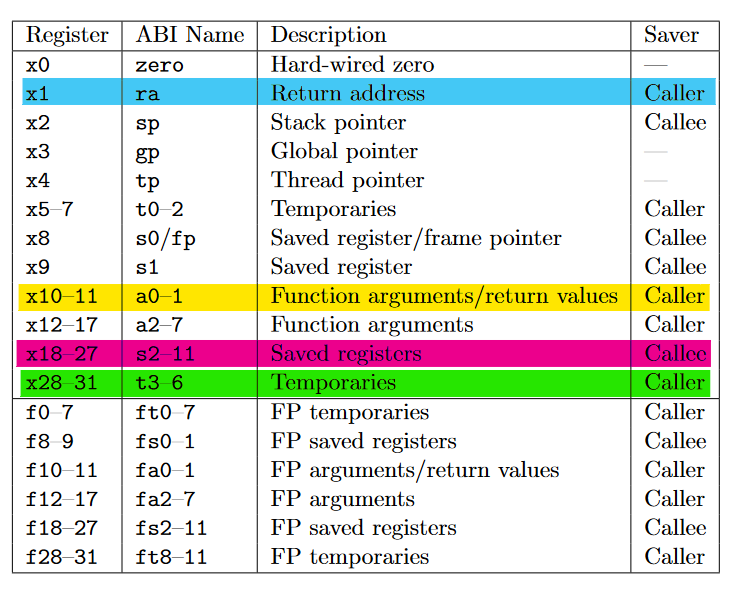
\includegraphics[width=\linewidth]{w03_calling_conv_regs.png}
	  \end{column}
	\end{columns}
  \end{frame}
  
  \begin{frame}[c]{Calling Convention - Argumentübergabe}                                    
	\begin{itemize}
	  \item Datentypen kleiner als 32-Bit werden auf 32-Bit Sign-extended
	  \item 64-Bit Werte in zwei a-Registern pro Wert, aufsteigend sortiert, untere Bit in niedrigerem Register
	  \item >64 Bit werden als Pointer übergeben
	  \item Weitere Parameter werden über den Stack übergeben
	  \item Stack muss immer 16-Byte aligned sein
   \end{itemize}                                          
  \end{frame}

  \begin{frame}[c]{Unterprogrammaufrufe in RISC-V}
	\begin{columns}[c]
	  \begin{column}{0.5\textwidth}
		Allgemeine Vorgehensweise:\\[.2cm] 
		\begin{enumerate}
		  \item Register sichern, Parameter vorbereiten
		  \item Sprung (Jump and Link)
		  \item Operation
		  \item Rücksprung (Jump (and Link) Register)
		\end{enumerate}
	  \end{column}
	  \begin{column}{0.4\textwidth}
		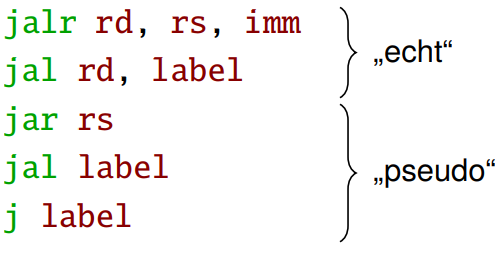
\includegraphics[width=\linewidth]{w03_jumpInstructionsWithPseudo_zue.png}
	  \end{column}
	\end{columns}
  \end{frame}
  
  \begin{frame}[c, fragile]{Rekursion: Schema}{}
	\begin{enumerate}
	  \item Basisfall (Abbruchbedingung) prüfen
		\begin{itemize}
		  \item Wenn ja --> vordefinierten Wert zurückgeben
		  \item Wenn nein --> weiter mit rekursiver Berechnung
		\end{itemize}
	  \item Sicherung von \verb|ra| und evtl. Parametern
	  \item Vorbereitung der Parameter für den rekursiven Aufruf
	  \item Rekursiver Aufruf
	  \item Ergebnis des Aufrufs verwerten
	  \item Wiederherstellung von \verb|ra|, \verb|sp|
	  \item Rücksprung
	\end{enumerate}
  \end{frame}
  
  \begin{frame}[c, fragile]{Rekursion: Beispiel}{}
	\begin{columns}[c]
	  \begin{column}{0.4\textwidth}
		\begin{lstlisting}[
		  basicstyle=\ttfamily,
		  numbers=left,
		  stepnumber=1,
		  showstringspaces=false,
		  tabsize=4,
		  breaklines=true,
		  breakatwhitespace=false,
		  frame=single,
		]
  fun:
	addi sp, sp, -8
	sw ra, 0(sp)
	sw a0, 4(sp)
	beq a0, zero, end
	addi a0, a0, -1
	jal fun
	end:
	lw ra, 0(sp)
	addi sp, sp, 8
	jalr zero, 0(ra)
		\end{lstlisting}
		\small \textbf{Achtung}: 8 Byte nicht CC-konform, nur zur besseren Darstellung
	  \end{column}
	  \begin{column}{0.5\textwidth}
		Aufruf mit {\ttfamily a0 = 3}:
		\vspace{2cm}
	  \end{column}
	\end{columns}
  \end{frame}
  
  
  \begin{frame}[c, fragile]{Rekursion: Beispiel}{}
	\begin{columns}[c]
	  \begin{column}{0.4\textwidth}
		\begin{lstlisting}[
		  basicstyle=\ttfamily,
		  numbers=left,
		  stepnumber=1,
		  showstringspaces=false,
		  tabsize=4,
		  breaklines=true,
		  breakatwhitespace=false,
		  frame=single,
		]
  fun:
	addi sp, sp, -8
	sw ra, 0(sp)
	sw a0, 4(sp)
	beq a0, zero, end
	addi a0, a0, -1
	jal fun
	end:
	lw ra, 0(sp)
	addi sp, sp, 8
	jalr zero, 0(ra)
		\end{lstlisting}
		\small \textbf{Achtung}: 8 Byte nicht CC-konform, nur zur besseren Darstellung
	  \end{column}
	  \begin{column}{0.5\textwidth}
		Aufruf mit {\ttfamily a0 = 3}:
		\begin{center}
		  \begin{tikzpicture}[scale=0.8]
			\def\stackwidth{2.5}
			\def\stackheight{0.6}
			\def\cellheight{0.6}
			\def\cellwidth{2.5}
  
			\foreach \slide/\vala/\valb in {1/0x3/ra, 2/0x2/ra, 3/0x1/ra, 4/0x0/ra} {
				\only<\slide->{
				  \draw (0,-\slide*2*\stackheight+\stackheight) rectangle ++(\stackwidth, -\cellheight) node[midway] {\texttt{\vala}};
				  \draw (0,-\slide*2*\stackheight) rectangle ++(\stackwidth, -\cellheight) node[midway] {\texttt{\valb}};
				}
				\only<\slide>{
				  \draw[<-, ultra thick] (\stackwidth+0.2, -\slide*2*\stackheight-\stackheight) -- ++(1,0) node [right] {\ttfamily{sp}};
				}
			  }
  
			\foreach \x/\vala/\valb in {1/ffff/fffb, 2/fff7/fff3, 3/ffef/ffeb, 4/ffe7/ffe3} {
			  \only<\x->{
				\node[anchor=east] at (-0.2, -\x*2*\stackheight+\stackheight - \cellheight/2) {\texttt{0x\vala}};
				\node[anchor=east] at (-0.2, -\x*2*\stackheight - \cellheight/2) {\texttt{0x\valb}};
			  }
			  } 
  
			\foreach \slide/\y in {5/2, 6/4, 7/6, 8/8}{
				\only<\slide>{
				  \draw[pattern=north east lines, pattern color=red] (0,-9*\stackheight) rectangle ++(\stackwidth, \y*\stackheight);
				  \draw[<-, ultra thick] (\stackwidth+0.2, \y*\stackheight-9*\stackheight) -- ++(1,0) node [right] {\ttfamily{sp}};
				}
			  }
		  \end{tikzpicture}
		\end{center}
	  \end{column}
	\end{columns}
  \end{frame}

% Caches  

\begin{frame}[fragile, c]{Caches: Zusammengefasst}{}
	\begin{itemize}
	  \item Zugriffe auf Hauptspeicher ($\equiv$ RAM) sind \textbf{extrem} langsam. Lösung: Caches
	  \item \enquote{Zwischenstation} zwischen Registern (sehr schnell, sehr klein) und Hauptspeicher (sehr langsam, sehr groß)
	  \item Miss-Latency, Hit-Latency, Miss-Penalty = Miss-Latency - Hit-Latency
	  \item \textbf{zeitliche Lokalität}: Zugriff auf x $\rightarrow$ wschl. Zugriff auf x in Zukunft
	  \item \textbf{räumliche Lokalität}: Zugriff auf x $\rightarrow$ wschl. Zugriff auf Nähe von x in Zukunft
	  \item Cold Miss, Conflict Miss, Capacity Miss
	\end{itemize}
\end{frame}


\begin{frame}[c]{Klassifikation von Misses}{}
	\resizebox{\textwidth}{!}{
		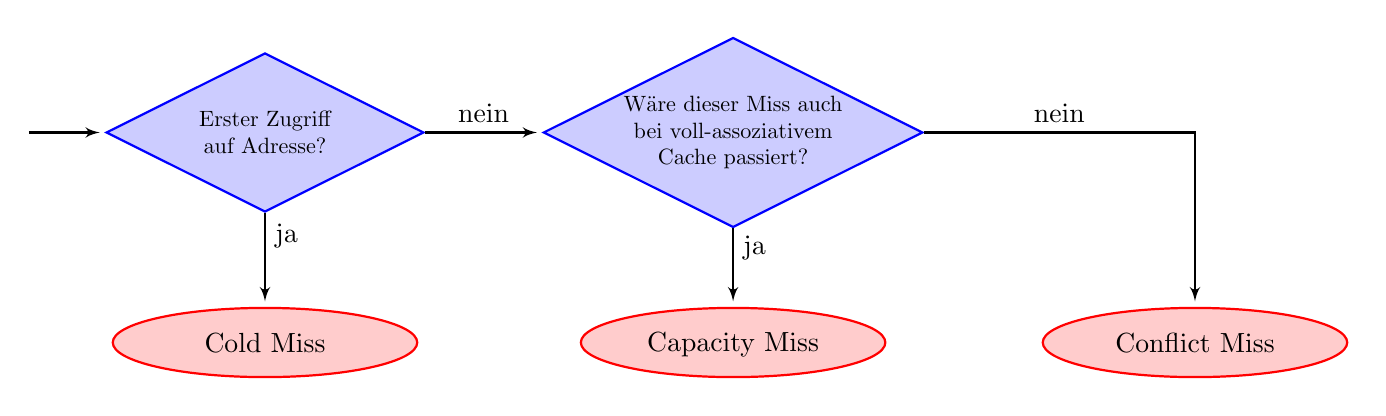
\begin{tikzpicture}
			[auto,
			ampersand replacement=\&,
			decision/.style={diamond, draw=blue, thick, fill=blue!20, text width=35mm, align=center, inner sep=1pt, scale=0.8, aspect=2},
			line/.style={draw, thick, -latex',shorten >=2pt},
			cloud/.style={draw=red, thick, ellipse,fill=red!20,
				minimum height=2.5em, text width=25mm, align=center, text depth=0pt}]
			
			\matrix [column sep=15mm,row sep=10mm]
			{
				\node [decision] (iscoldmiss) {Erster Zugriff auf Adresse?};
				\& \node [decision] (iscapmiss) {Wäre dieser Miss auch bei voll-assoziativem Cache passiert?}; \&\\
				\node [cloud] (coldmiss) {Cold Miss};
				\& \node [cloud] (capacitymiss) {Capacity Miss};
				\& \node [cloud] (conflictmiss) {Conflict Miss};\\
			};
			\begin{scope}[every path/.style=line]
				\path (iscoldmiss) + (left:30mm) -- (iscoldmiss);
				\path (iscoldmiss) -- node [near start] {ja} (coldmiss);
				\path (iscoldmiss) -- node [midway] {nein} (iscapmiss);
				\path (iscapmiss)  -- node [near start] {ja} (capacitymiss);
				\path (iscapmiss)  -| node [near start] {nein} (conflictmiss);
			\end{scope}
	\end{tikzpicture}}
\end{frame}
  
\begin{frame}
	\frametitle{Messung der Cache-Güte}
	\vfill
	\begin{equation*}
	  \text{CPU Time} = \text{IC} \cdot \left(\dfrac{\text{CPI}}{f} + \frac{\text{Memory Accesses}}{\text{Instruction}} \cdot \text{Average Memory Access Time}\right)
	\end{equation*}
	\begin{equation*}
	  \text{Average Memory Access Time} = \text{Hit Rate} \cdot \text{Hit Latency} + \text{Miss Rate} \cdot \text{Miss Latency}
	\end{equation*}
	\vfill
	{\renewcommand{\arraystretch}{1.4}
		\begin{tabular}{rl}
			Frequenz ($f$): & Frequenz des Prozessors\footnote{für uns in der Einheit $\frac{\text{cycles}}{\text{s}}$}\\
			Instruction Count (IC): & Anzahl an auszuführenden Instruktionen\\
			Cycles per Instruction (CPI): & (Durchschnitts-) Anzahl an Zyklen pro Instruktion\\
			Memory Access Rate: & (Durchschnitts-) Anzahl an Speicherzugriffen pro Instruktion\\
	\end{tabular}}
\end{frame}
  
\begin{frame}[c]{Cachearten: Direct Mapped Cache}{}
	\begin{columns}[c]
	  \begin{column}{0.5\textwidth}
		\begin{itemize}
		  \item Ein Datum wird auf genau eine Cachezeile gemapped
		  \item möglicherweise sehr viele Verdrängungen
		  \item Nur ein Tag-Vergleich notwendig $\rightarrow$ effizienter Zugriff
		  \item \#Offsetbits = log2(Cachezeilenlänge)
		  \item \#Indexbits = log2(Anzahl Cachelines)
		  \item \#Tagbits = Adresslänge - \#Indexbits - \#Offsetbits
		\end{itemize}
	  \end{column}
	  \begin{column}{0.5\textwidth}
		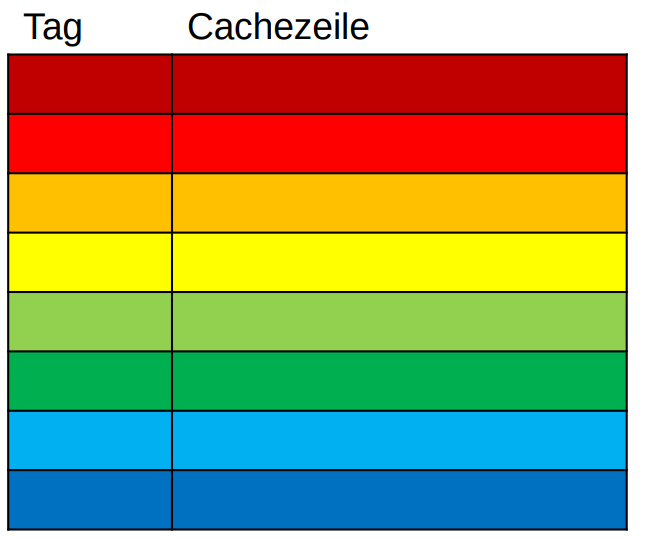
\includegraphics[width=\linewidth]{w05_directmapped_rep.png}
	  \end{column}
	\end{columns}
\end{frame}
  
\begin{frame}[c]{Cachearten: Vollassoziativer Cache}{}
	\begin{columns}[c]
	  \begin{column}{0.5\textwidth}
		\begin{itemize}
		  \item Datum hat keine feste Position im Cache
		  \item Im Worst-Case müssen bei Zugriff alle Zeilen durchlaufen werden, um Tag zu vergleichen $\rightarrow$ ineffizient
		  \item \#Offsetbits = log2(Cachezeilenlänge)
		  \item \#Indexbits = 0
		  \item \#Tagbits = Adresslänge - \#Offsetbits
		\end{itemize}
	  \end{column}
	  \begin{column}{0.5\textwidth}
		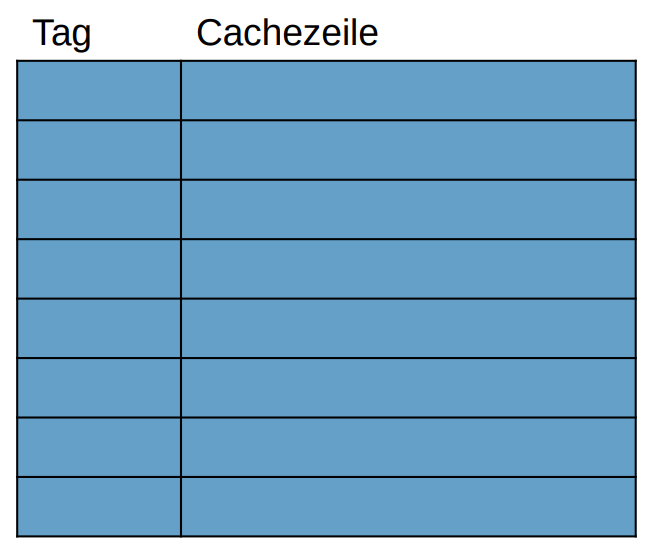
\includegraphics[width=\linewidth]{w05_vollassoz_rep.png}
	  \end{column}
	\end{columns}
\end{frame}
  
\begin{frame}[c]{Cachearten: Mengenassoziativer Cache}{}
	\begin{columns}[c]
	  \begin{column}{0.5\textwidth}
		\begin{itemize}
		  \item Ein Datum wird auf eine Teilmenge der Cachezeilen gemapped (Index) 
		  \item Bei Zugriff nur Tag-Vergleiche innerhalb des Sets $\rightarrow$ relativ effizienter Zugriff 
		  \item weniger Verdrängungen als beim Direct-Mapped
		  \item \#Offsetbits = log2(Cachezeilenlänge)
		  \item \#Indexbits = log2(Anzahl Cache\textbf{sets})
		  \item \#Tagbits = Adresslänge - \#Indexbits - \#Offsetbits
		\end{itemize}
	  \end{column}
	  \begin{column}{0.5\textwidth}
		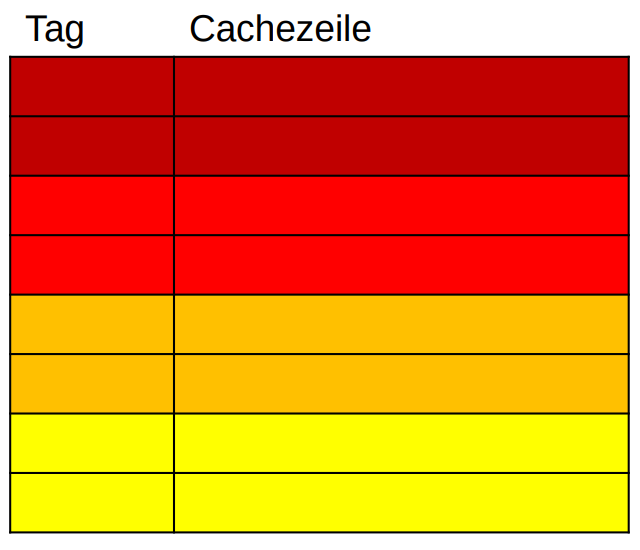
\includegraphics[width=\linewidth]{w05_mengenassoz_rep.png}
	  \end{column}
	\end{columns}
\end{frame}

\begin{frame}[c]{Adressierung}
	\begin{itemize}
		\item 4-fach-assoziativer Cache
		\item Cachegröße: 128 Byte
		\item Cachezeile: 4 Byte
	\end{itemize}
	\vspace{-1ex}
	\begin{center}
  \resizebox{.7\textwidth}{!}{
  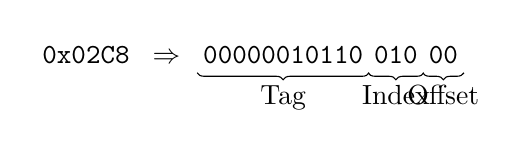
\begin{tikzpicture}[ampersand replacement=\&]
	\matrix (cache) [matrix of nodes, nodes={minimum height=1em, inner xsep=2pt, font={\ttfamily}}]
	{
	  0x02C8 \&[1ex] \(\Rightarrow\) \&[1ex] 00000010110 \& 010 \& 00 \&[1ex] \\
	};
	\draw<1> [decorate, decoration = {brace, mirror}] (cache-1-5.south west) -- node[below,midway,inner ysep=1ex]{Offset} (cache-1-5.south east);
	\draw<2> [decorate, decoration = {brace, mirror}] (cache-1-4.south west) -- node[below,midway,inner ysep=1ex]{Index} (cache-1-4.south east);
	\draw<3> [decorate, decoration = {brace, mirror}] (cache-1-3.south west) -- node[below,midway,inner ysep=1ex]{Tag} (cache-1-3.south east);
  \end{tikzpicture}
  }
  \end{center}
  \vspace{-1ex}
  \only<1>{\textbf{Offset Bits} -- bezeichnen das Byte der Cachezeile, auf das zugegriffen werden soll. \\Die Cachezeilengröße ist in unserem Beispiel 4 Bytes, deswegen genügen $\log_2{4}=2$ Bits.}
  
  \only<2>{\textbf{Index Bits} -- bestimmen das Cache-Set, in dem die gewählte Adresse sein kann. \\In unserem Beispiel ist der Cache 128 Byte groß, hat eine Cachezeilen-Größe von 4 Byte und ist 4-fach-assoziativ. Also es gibt $\frac{\frac{128}{4}}{4} = 8$ Sets. Daher benötigt man hier $\lceil\log_2{8}\rceil = 3$ Bits. Die Daten werden also in Set \#2 landen.}
  
  \only<3>{\textbf{Tag Bits} -- restliche Bits. Identifizieren die in einer Cachezeile gespeicherten Daten eindeutig.}
\end{frame}
  
\begin{frame}[c]{Aufgabe: Cache-Bits-Berechnung}{}
	Auf einer 32-Bit Architektur sei ein Cache von 32 Byte mit 4 Byte Cachezeilenlänge gegeben:
	\vspace{0.5cm}
	\begin{itemize}
		\item Wieviele Cachelines gibt es?
		\item Gib die Anzahl an Tag-, Index- und Offsetbits an, wenn Cache direct-mapped ist
		\item Gib die Anzahl an Tag-, Index- und Offsetbits an, wenn Cache vollassoziativ ist
		\item Gib die Anzahl an Tag-, Index- und Offsetbits an, wenn Cache 4-fach-assoziativ ist
	\end{itemize}
\end{frame}

\begin{frame}[c]{Lösung: Cache-Bits-Berechnung}{}
	Auf einer 32-Bit Architektur sei ein Cache von 32 Byte mit 4 Byte Cachezeilenlänge gegeben:
	\vspace{0.5cm}
	\begin{itemize}
		\item Wieviele Cachelines gibt es?
		\begin{itemize}
			\item 32/4 = 8 Cachelines
		\end{itemize}
		\item Gib die Anzahl an Tag-, Index- und Offsetbits an, wenn Cache direct-mapped ist
		\begin{itemize}
			\item Index = log2(8) = 3, Offset = log2(4) = 2, Tag = 32 - 2 - 3 = 27
		\end{itemize}
		\item Gib die Anzahl an Tag-, Index- und Offsetbits an, wenn Cache vollassoziativ ist
		\begin{itemize}
			\item Index = 0, Offset = log2(4) = 2, Tag = 32 - 2 = 30
		\end{itemize}
		\item Gib die Anzahl an Tag-, Index- und Offsetbits an, wenn Cache 4-fach-assoziativ ist
		\begin{itemize}
			\item Index = log2(2) = 1, Offset = log2(4) = 2, Tag = 32 - 2 - 1 = 29
		\end{itemize}
	\end{itemize}
\end{frame}

\begin{frame}[c]{Aufgabe: Cache-Mapping}{}
	Gegeben sei ein Cache von 32 Byte mit 4 Byte Cachezeilenlänge. Auf wieviele Cachezielen kann das Datum 0x7 gemapped werden, wenn
	\vspace{0.5cm}
	\begin{itemize}
		\item der Cache vollassoziativ ist?
		\item der Cache 4-fach assoziativ ist?
		\item der Cache direct-mapped ist?
	\end{itemize}
\end{frame}

\begin{frame}[c]{Lösung: Cache-Mapping}{}
	Gegeben sei ein Cache von 32 Byte mit 4 Byte Cachezeilenlänge. Auf wieviele Cachezielen kann das Datum 0x7 gemapped werden, wenn
	\vspace{0.5cm}
	\begin{itemize}
		\item der Cache vollassoziativ ist?
		\begin{itemize}
			\item Auf alle, also 8
		\end{itemize}
		\item der Cache 4-fach assoziativ ist?
		\begin{itemize}
			\item Auf ein Cacheset, also 4
		\end{itemize}
		\item der Cache direct-mapped ist?
		\begin{itemize}
			\item Auf eine Zeile, also 1
		\end{itemize}
	\end{itemize}
\end{frame}

\begin{frame}[c]{Wiederholung}{}
	\begin{center}
	  \LARGE Single Cycle + Prozessorerweiterungen
	\end{center}
\end{frame}


\begin{frame}[c, fragile]{Prozessor-Komponenten}{}
	\begin{center}
		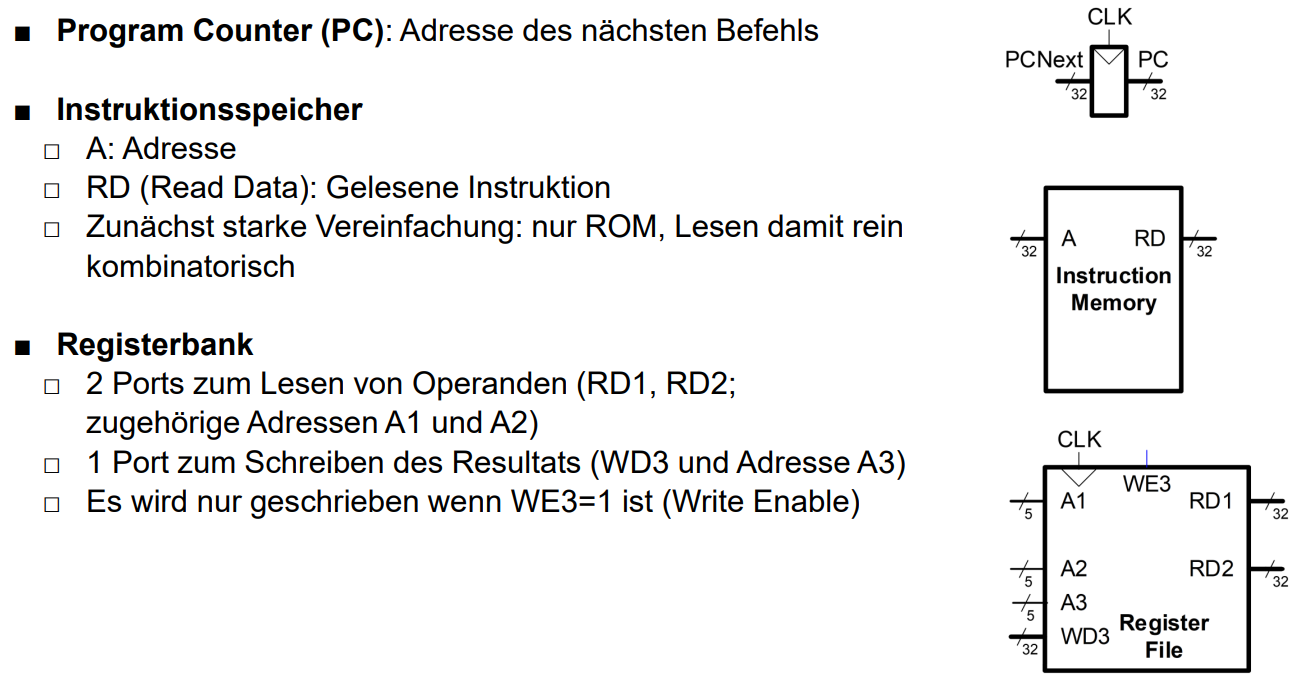
\includegraphics[width=0.85\textwidth]{w08_prozessorcomponents1_lv.png}
	\end{center}
\end{frame}

\begin{frame}[c, fragile]{Prozessor-Komponenten}{}
	\begin{center}
		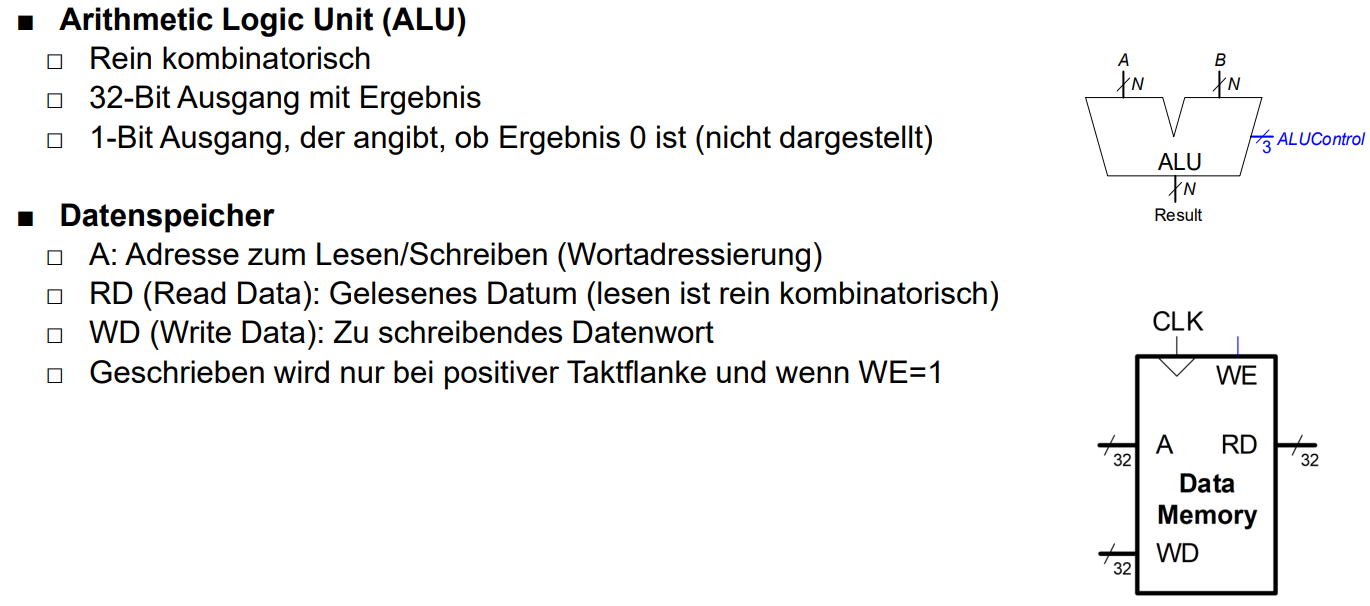
\includegraphics[width=0.85\textwidth]{w08_prozessorcomponents2.png}
	\end{center}
\end{frame}

\begin{frame}[c, fragile]{Single-Cycle-Prozessor Signale}{}
	\begin{itemize}
		\item \textbf{PCSrc}: Nächste Instruktion (+4) oder Sprung-Adresse
		\item \textbf{Zero}: 1 wenn das ALU-Ergebnis = 0 ist
		\item \textbf{Jump}: Ist Instruktion ein unbedingter-Sprung
		\item \textbf{Branch}: Ist Instruktion ein bedingter-Sprung
		\item \textbf{ResultSrc}: Was soll ins Register geschrieben werden
		\item \textbf{MemWrite}: Soll in Memory geschrieben werden
		\item \textbf{ALUControl}: Welche arithmetische Operation
		\item \textbf{ALUSrc}: Immediate oder Register in ALU
		\item \textbf{ImmSrc}: Welche Bits sind der Immediate
		\item \textbf{RegWrite}: Soll in Register-File geschrieben werden
	\end{itemize}
\end{frame}

\begin{frame}[c]{RISC-V Single-Cycle-Prozessor}{}
	\begin{center}
		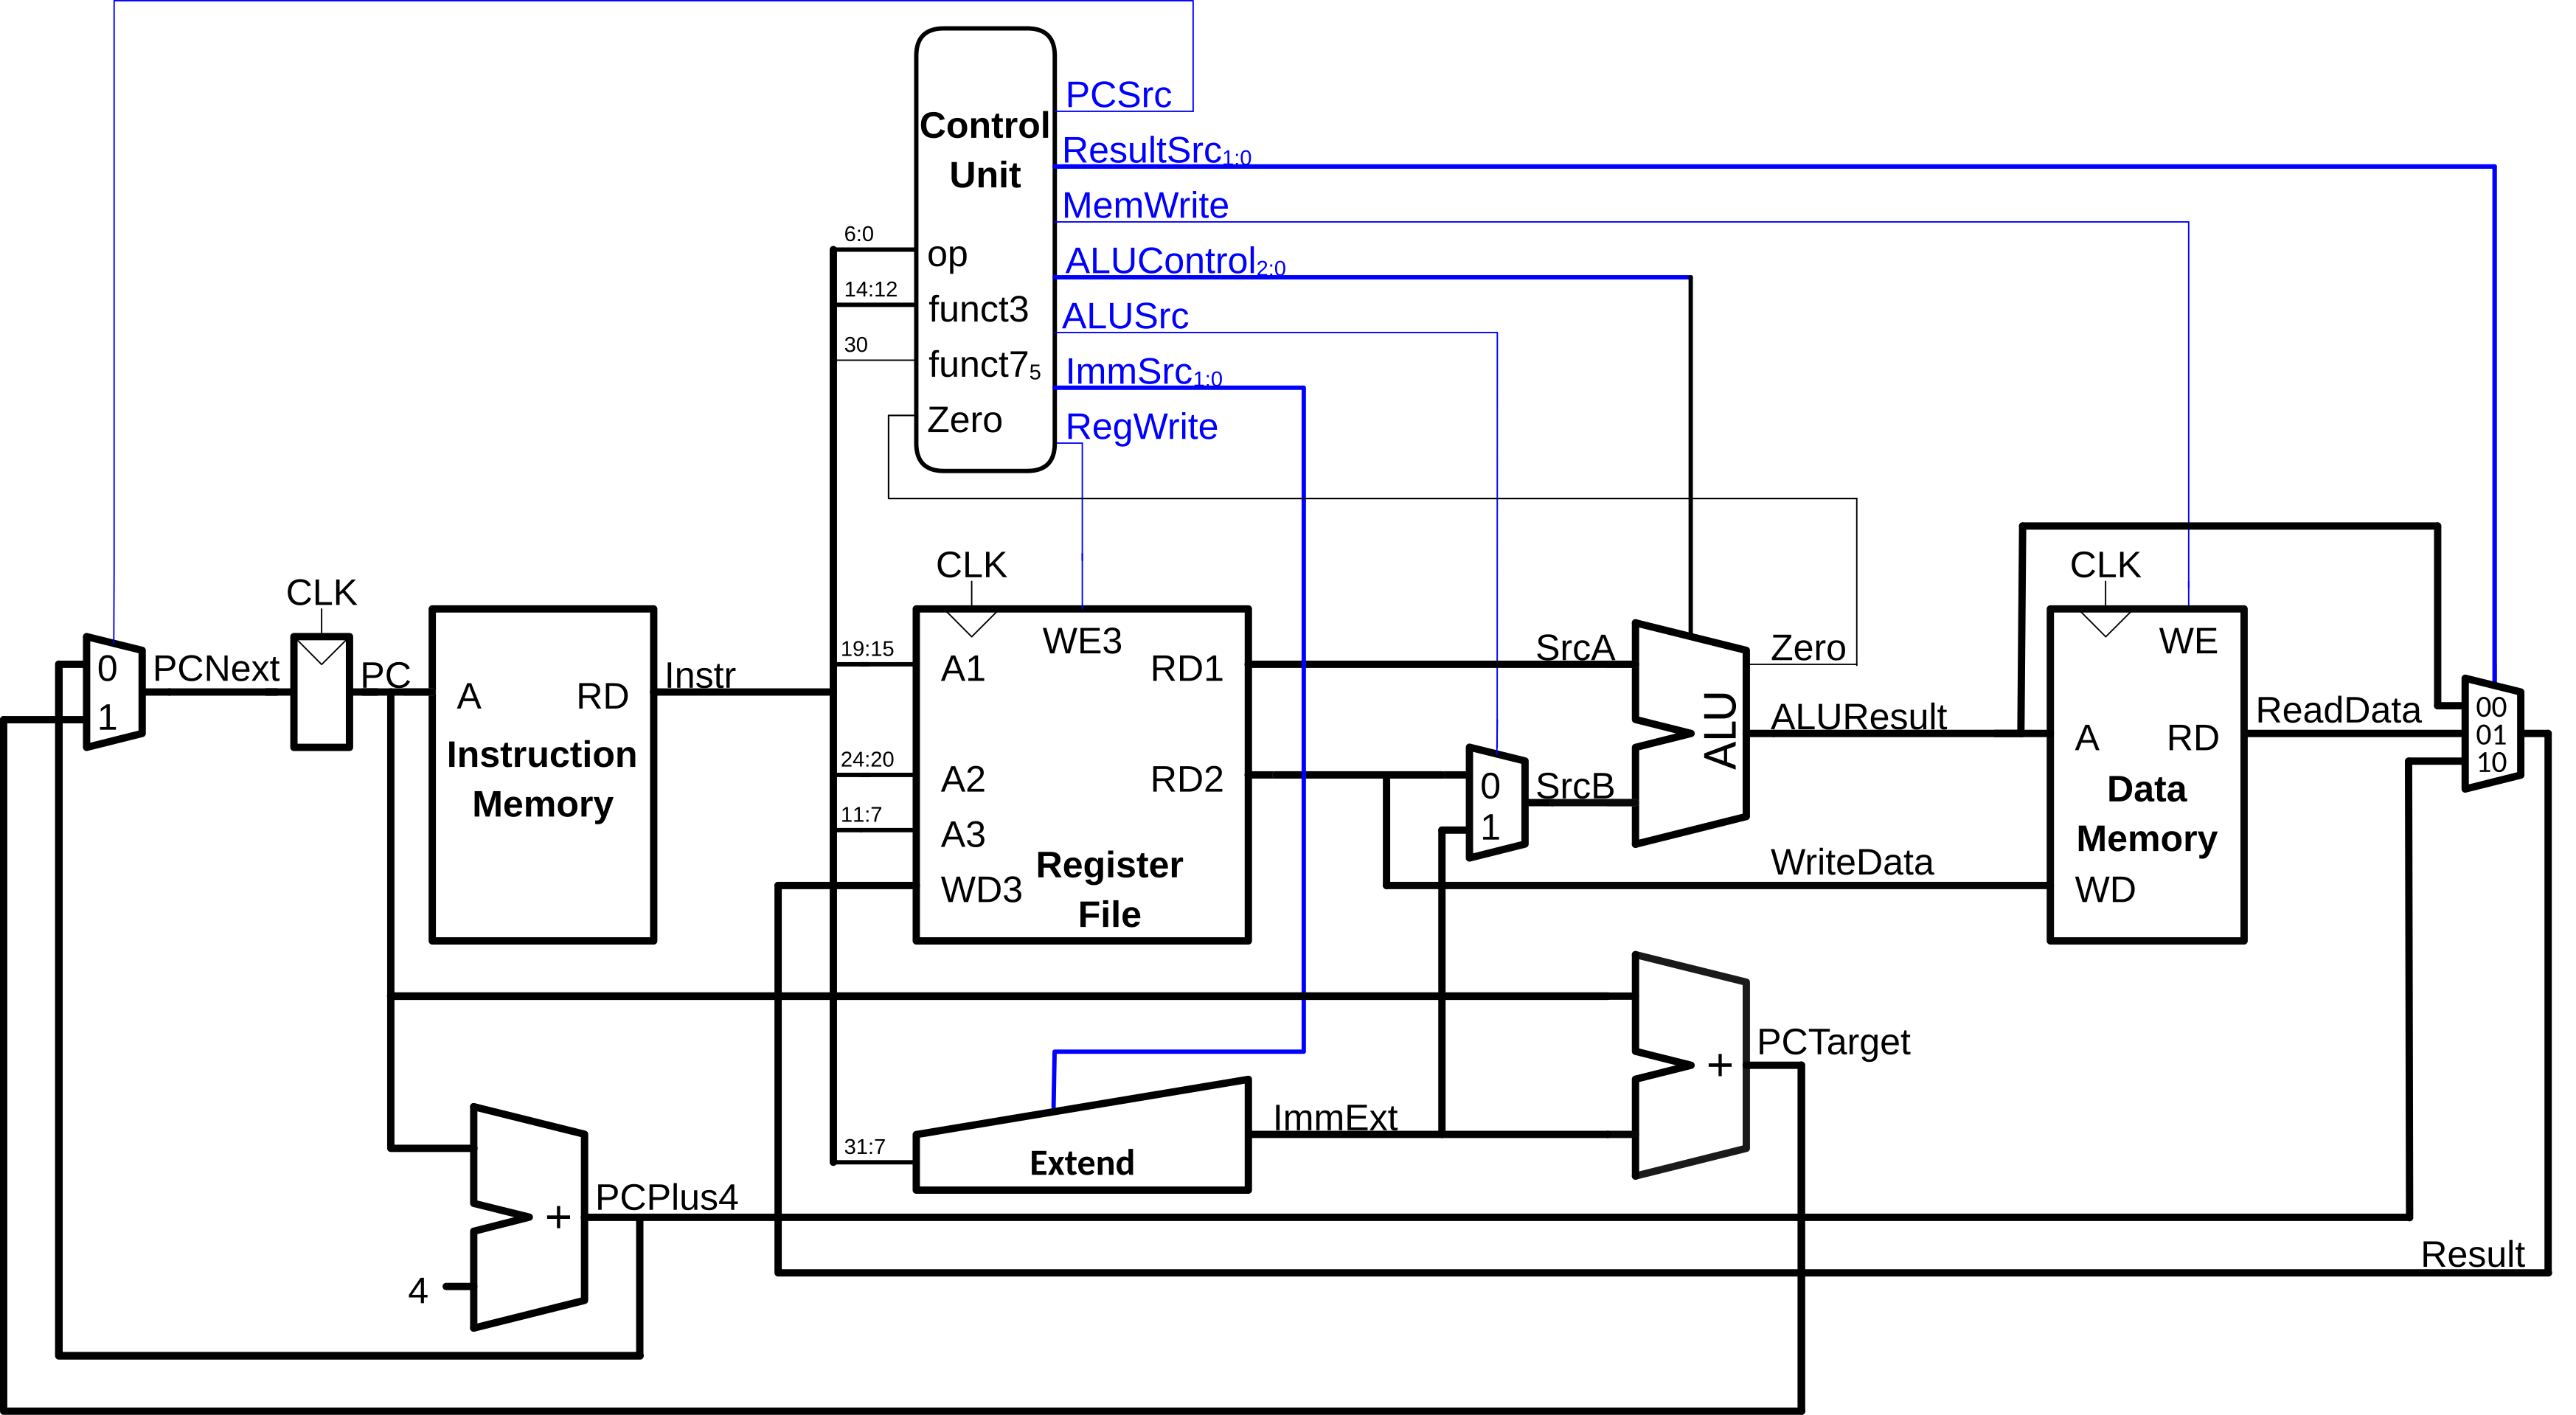
\includegraphics[width=0.79\textwidth]{w08_single_cycle.png}
	\end{center}
	\centering
	\tiny (Quelle: Vorlesungsmaterialien ERA)
\end{frame}

\begin{frame}[c, fragile]{Herangehensweise bei Erweiterungen}{}
	\begin{itemize}
		\item Naive Idee (nicht in Klausur anwenden)
		\begin{itemize}
			\item Befehl komplett neu implementieren
			\item Zeitaufwändig und kompliziert, da im schlimmsten Fall alle Module verändern
		\end{itemize}
		\item Besserer Versuch: bestehende Funktionalität anpassen
		\begin{itemize}
			\item Bestehender Befehl, der am ähnlichsten ist suchen
			\item Unterschiede in Funktionalität feststellen
			\item Mittels Gatter beide Befehle unterscheiden (opcode, funct3, funct7)
			\item Danach schauen, dass keine anderen Befehle verändert wurden	
		\end{itemize}
	\end{itemize}
\end{frame}


\begin{frame}[c]{Aufgabe: Prozessorerweiterung}{}
	Erweitere den dir bekannten RISC-V Single-Cycle Prozessor, dass er auch die \textbf{lbu}-Instruktion unterstützt. Zeichne dabei das veränderte Schaltbild und möglicherweise veränderte Control-Unit Signale ein. Falls du neue Komponenten benötigst zeichne auch deren Schaltbild.
	\vspace{0.5cm}
	\begin{columns}[c]
		\begin{column}{0.5\textwidth}
			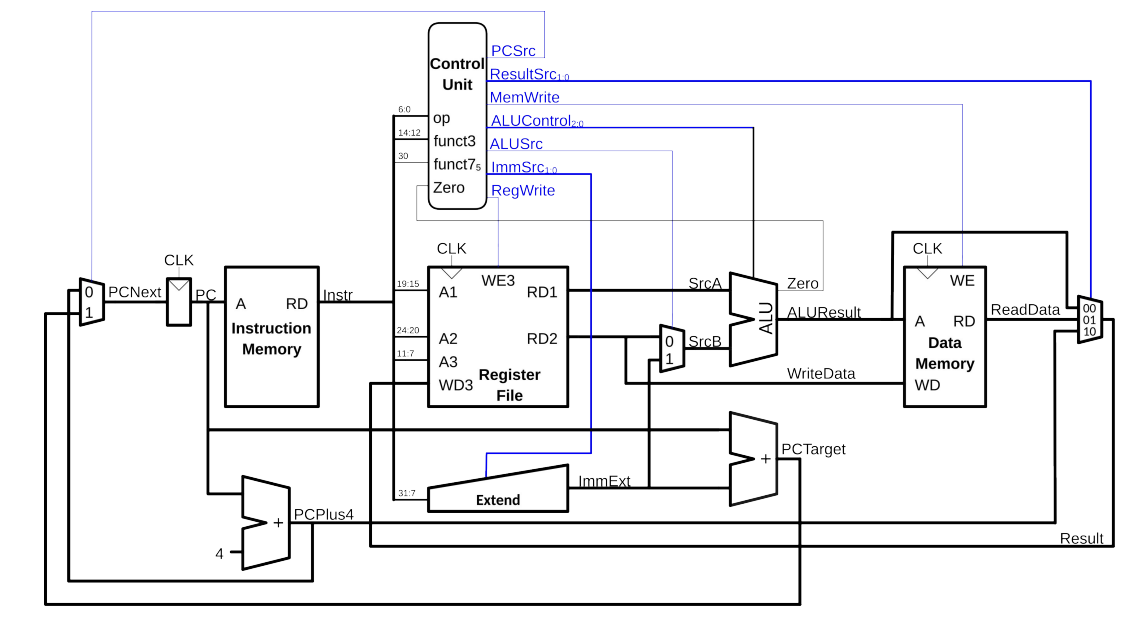
\includegraphics[width=1.0\textwidth]{w06_singlecycleriscv_lv.png}
		\end{column}
		\begin{column}{0.5\textwidth}
			\begin{center}
				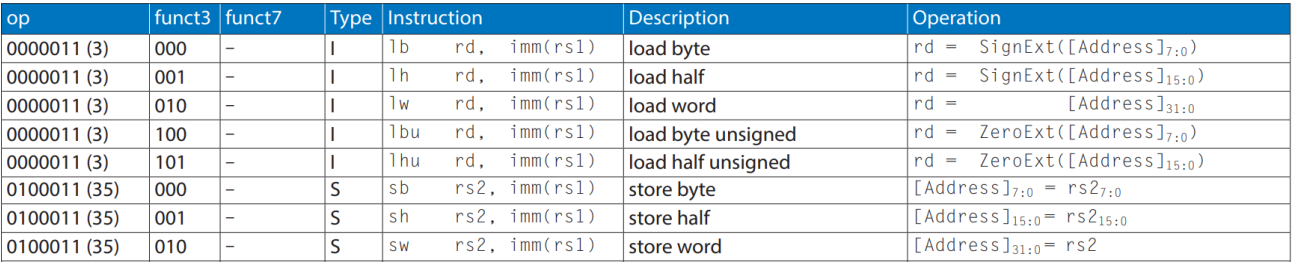
\includegraphics[width=1.0\textwidth]{w03_loadbefehle.png}
			\end{center}
		\end{column}
	\end{columns}
\end{frame}

\begin{frame}[c]{Lösung: Prozessorerweiterung}{}
	Erweitere den dir bekannten RISC-V Single-Cycle Prozessor, dass er auch die \textbf{lbu}-Instruktion unterstützt. Zeichne dabei das veränderte Schaltbild und möglicherweise veränderte Control-Unit Signale ein. Falls du neue Komponenten benötigst zeichne auch deren Schaltbild.
	\vspace{0.5cm}
	\begin{columns}[c]
		\begin{column}{0.5\textwidth}
			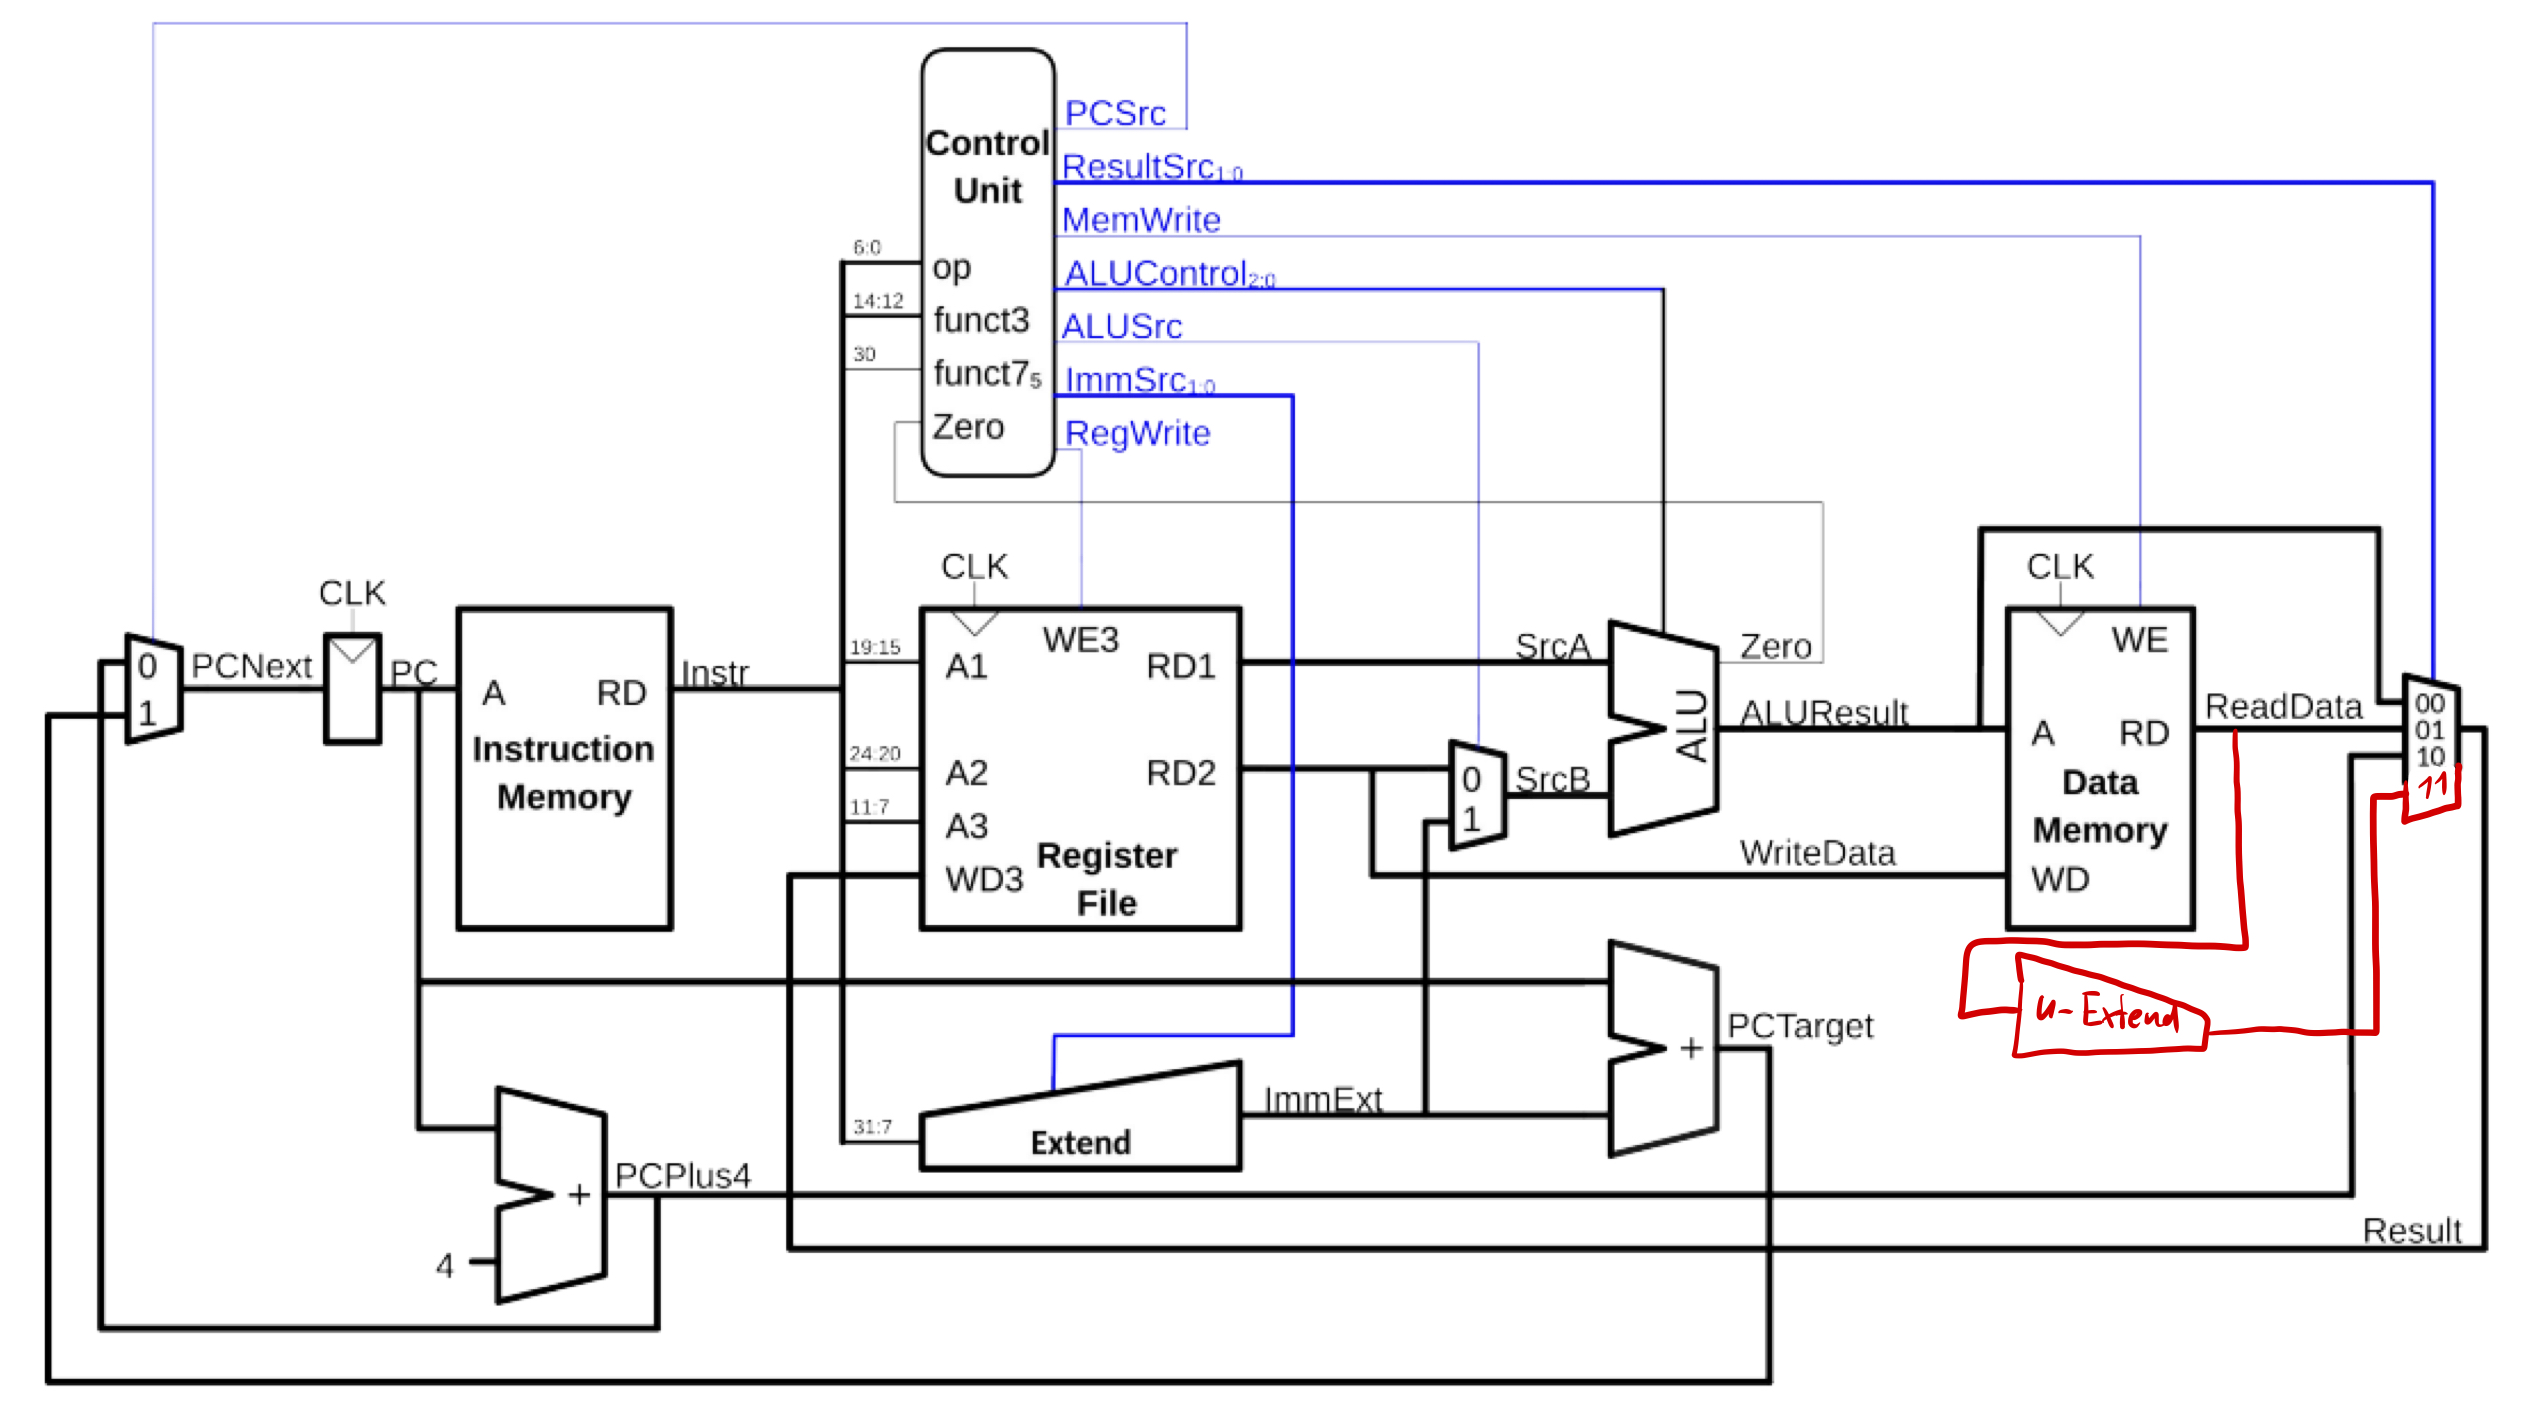
\includegraphics[width=1.0\textwidth]{w14_lbu_erweiterung.jpeg}
		\end{column}
		\begin{column}{0.5\textwidth}
			\begin{center}
				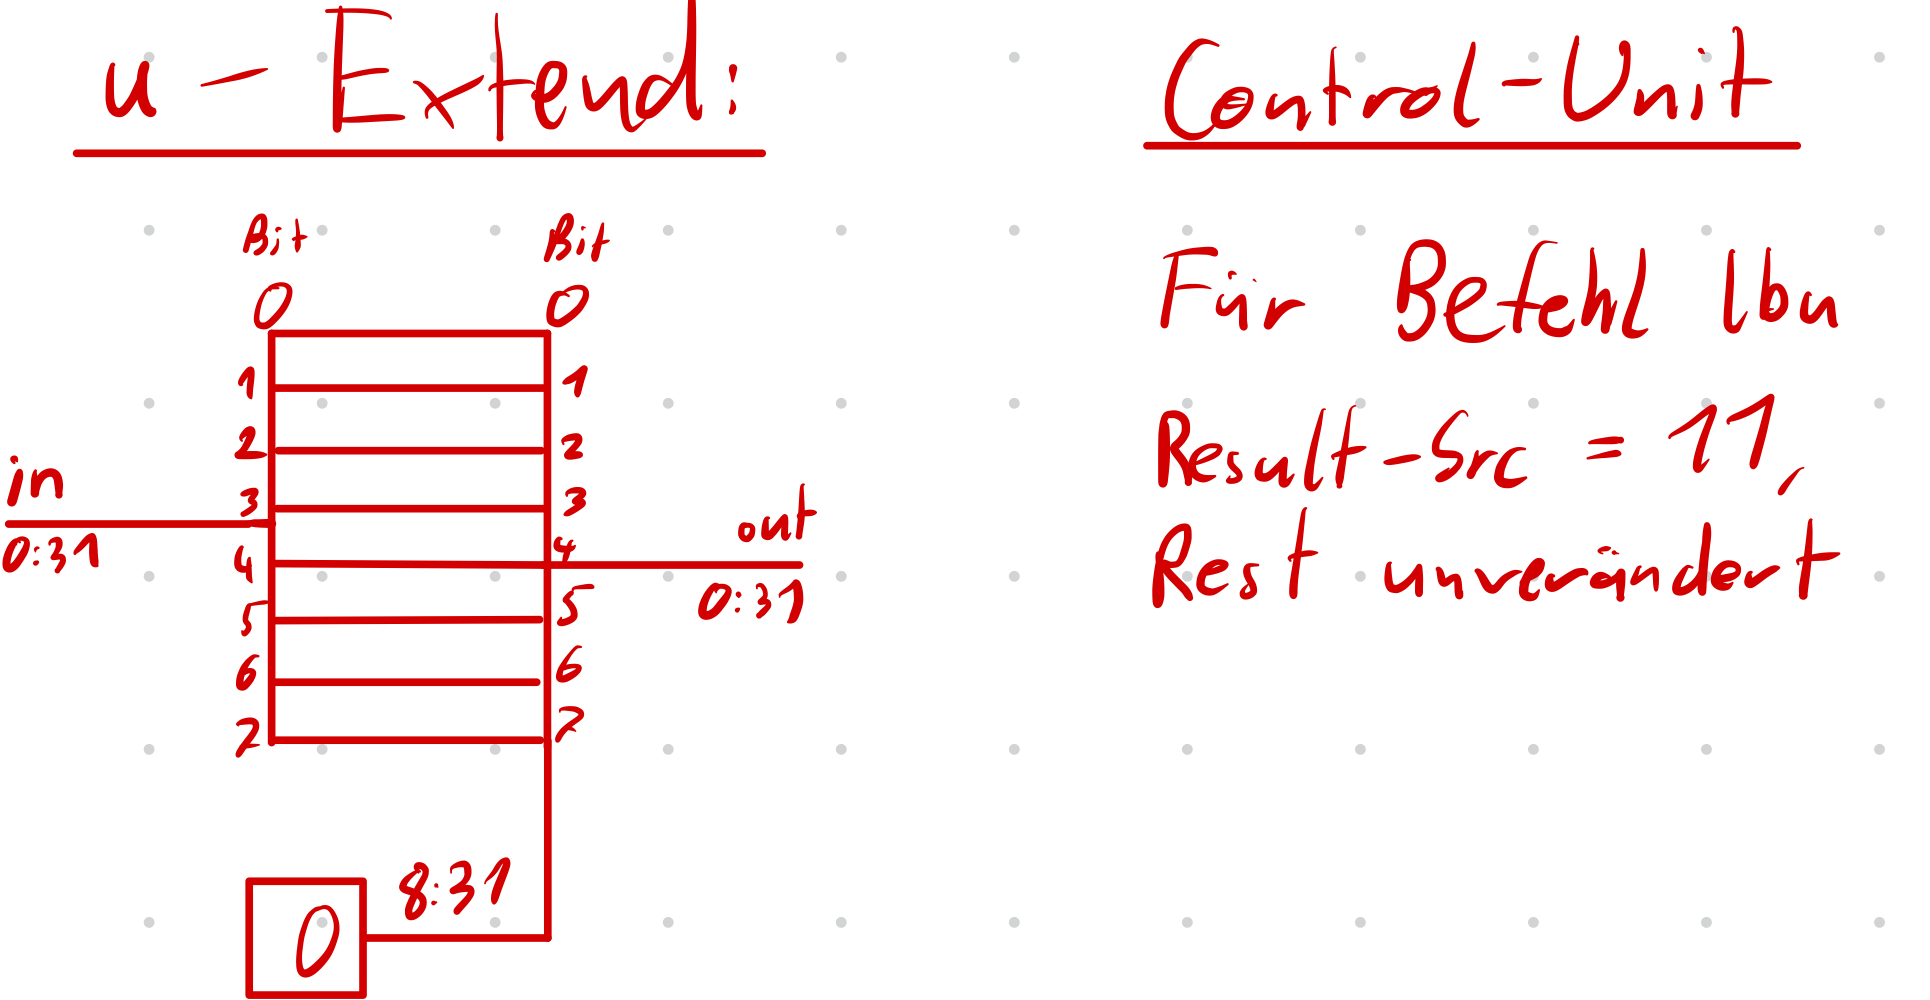
\includegraphics[width=0.9\textwidth]{w14_uextend.jpeg}
			\end{center}
		\end{column}
	\end{columns}
\end{frame}


% ---------- AUTO MATEN ---------------

\begin{frame}[c]{Wiederholung}{}
	\begin{center}
	  \LARGE Automaten
	\end{center}
\end{frame}

\begin{frame}[fragile, c]{Endliche Automaten}{}
	\begin{itemize}
		\item Repräsentiert Funktion einer sequentiellen Schaltung (sequentiell: zustandsabhängig)
		\item Mathematische Beschreibung als 6-Tupel $(I, O, S, s_0, \delta, \lambda)$:
		      \begin{itemize}
			      \item $I$: Menge möglicher Eingaben
			      \item $O$: Menge möglicher Ausgaben
			      \item $S$: Zustandsmenge
			      \item $s_0$: Startzustand
			      \item $\delta:  S\times I\rightarrow S$: Zustandsübergangsfunktion
			      \item $\lambda: S\rightarrow O$ (Moore), $\lambda: S\times I\rightarrow O$ (Mealy): Ausgabefunktion
		      \end{itemize}
      \item Als Diagramm:
        \begin{itemize}
          \item Zustände $\rightarrow$ Kreise
          \item Übergänge $\rightarrow$ Kanten
          \item Bedingungen $\rightarrow$ Kantenbeschriftungen
        \end{itemize}
	\end{itemize}
\end{frame}

\begin{frame}[fragile, c]{Endliche Automaten: Moore vs. Mealy}{}
	\begin{columns}[c]
		\begin{column}{0.5\textwidth}
			\begin{center}
				\textbf{Moore-Automat}\\
				{\scriptsize Ausgabe abhängig von aktuellem Zustand}\\
				\resizebox{!}{0.60\textheight}{
					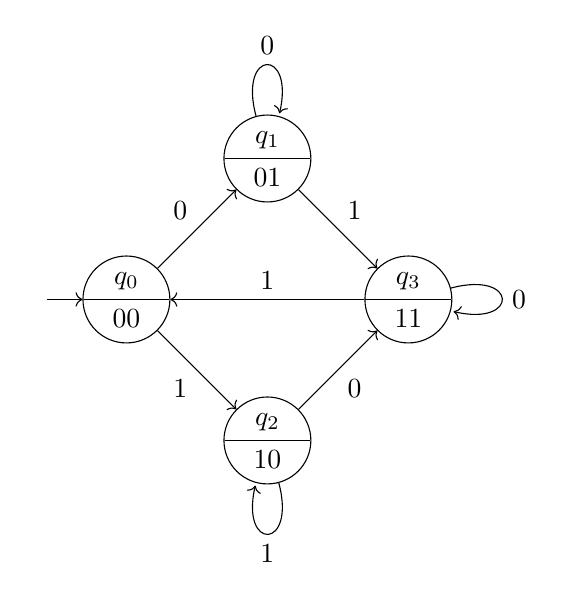
\begin{tikzpicture}[initial text=]
						\node[state with output, initial] (q0) {$q_0$  \nodepart{lower} $00$};
						\node[state with output] (q1) [above right=of q0] {$q_1$  \nodepart{lower} $01$};
						\node[state with output] (q2) [below right=of q0] {$q_2$  \nodepart{lower} $10$};
						\node[state with output] (q3)  [below right=of q1] {$q_3$  \nodepart{lower} $11$};

						\path[->, every node/.style={execute at begin node=$, execute at end node=$}]
						(q0) edge node [above left]  {0} (q1)
						edge node [below left]  {1} (q2)
						(q1) edge node [above right] {1} (q3)
						edge [loop above] node {0} ()
						(q2) edge node [below right] {0} (q3)
						edge [loop below] node {1} ()
						(q3) edge [loop right] node {0} ()
						(q3) edge node [above] {1} (q0);
					\end{tikzpicture}
				}
			\end{center}
		\end{column}
		\begin{column}{0.5\textwidth}
			\begin{center}
				\textbf{Mealy-Automat}\\
				{\scriptsize Ausgabe abhängig von aktuellem Zustand + Eingabe}\\
				\resizebox{!}{0.60\textheight}{
					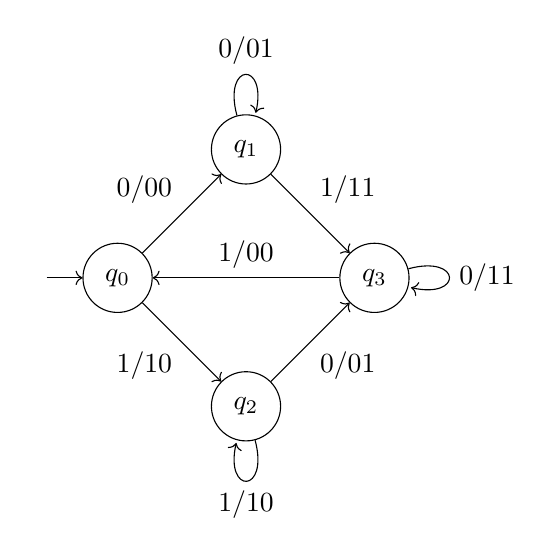
\begin{tikzpicture}[initial text=]
						\node[state, initial] (q0) {$q_0$  \nodepart{lower} $00$};
						\node[state] (q1) [above right=of q0] {$q_1$};
						\node[state] (q2) [below right=of q0] {$q_2$};
						\node[state] (q3)  [below right=of q1] {$q_3$};
						
						\path[->, every node/.style={execute at begin node=$, execute at end node=$}]
						(q0) edge node [above left]  {0/00} (q1)
						edge node [below left]  {1/10} (q2)
						(q1) edge node [above right] {1/11} (q3)
						edge [loop above] node {0/01} ()
						(q2) edge node [below right] {0/01} (q3)
						edge [loop below] node {1/10} ()
						(q3) edge [loop right] node {0/11} ()
						(q3) edge node [above] {1/00} (q0);
					\end{tikzpicture}
				}
			\end{center}
		\end{column}
	\end{columns}
	\begin{center}
		{\scriptsize $I=\{0, 1\}$, $O=\{00, 01, 10, 11\}$, $S=\{q_0, q_1, q_2, q_3\}, \delta, \lambda$ (abh. vom Typen)}
	\end{center}
\end{frame}

\begin{frame}[fragile, c]{Endliche Automaten: Implementierung}{}
	\begin{itemize}
		\item One-Hot-Kodierung: Genau 1 FF ist auf 1 $\rightarrow$ aktueller Zustand
      \begin{itemize}
        \item Kann direkt aus Automat umgesetzt werden, wird schnell unübersichtlich (viele Gatter)
      \end{itemize}
		\item Binärkodierung: FFs zusammen bilden Binärzahl des aktuellen Zustands
      \begin{itemize}
        \item Spart Gatter, ursprüngliche Funktionalität nicht mehr trivial am Schaltkreis ablesbar
      \end{itemize}
		\item Mikroprogrammierte Steuerwerke: Ein Speicherbaustein enthält vollständigen Automaten, Eingaben werden als Adressen interpretiert.
      \begin{itemize}
        \item Sehr flexibel
      \end{itemize}
  \end{itemize}
	\begin{table}[]
		\begin{tabular}{c|c|c}
			Zustand & One-Hot-Enkodierung & Binärkodierung \\ \hline
			$S_0$   & $0001$              & $00$             \\
			$S_1$   & $0010$              & $01$             \\
			$S_2$   & $0100$              & $10$             \\
			$S_3$   & $1000$              & $11$
		\end{tabular}
	\end{table}
\end{frame}

\begin{frame}[c]{One-Hot-Kodierung}{}
	\begin{center}
		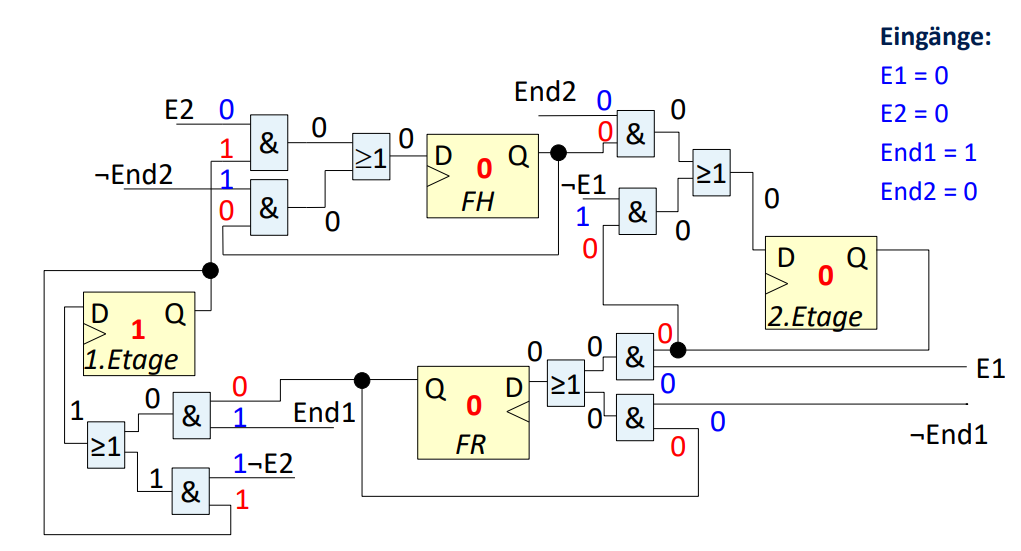
\includegraphics[width=0.73\textwidth]{w09_onehot_lv.png}
	\end{center}
	\centering
	\tiny (Quelle: Vorlesungsmaterialien ERA)
\end{frame}

\begin{frame}[c]{Binäre Kodierung}{}
  \begin{columns}[c]
		\begin{column}{0.5\textwidth}
      \begin{center}
        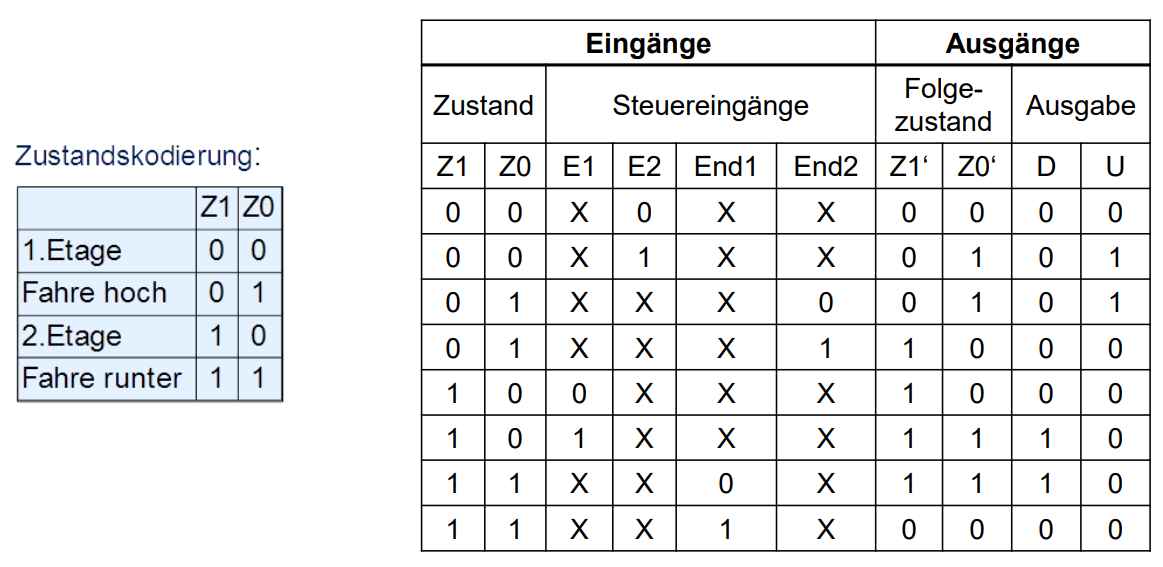
\includegraphics[width=\textwidth]{w09_bincode1_lv.png}
      \end{center}
    \end{column}
    \begin{column}{0.5\textwidth}
      \begin{center}
        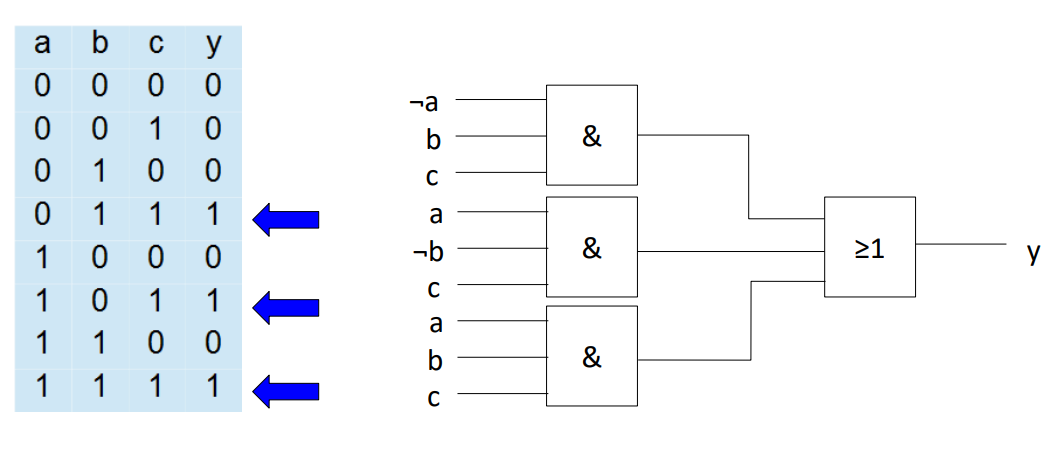
\includegraphics[width=\textwidth]{w09_bincode2_lv.png}
      \end{center}
    \end{column}
  \end{columns}
  \vspace{0.5cm}
	\centering
	\tiny (Quelle: Vorlesungsmaterialien ERA)
\end{frame}

\begin{frame}[c]{Wiederholung}{}
	\begin{center}
	  \LARGE Pipelining
	\end{center}
\end{frame}

\begin{frame}[fragile, c]{Pipelining}{}
	\begin{itemize}
		\item Parallele Verarbeitung von mehreren Instruktionen
		\item Aufteilung der Instruktionsverarbeitung in 5 Teilschritte: Fetch, Decode, Execute, Memory, Writeback
		\item Daten- und Kontrollpfad des Prozessors wird aufgeteilt: Register zur Zwischenspeicherung dazwischen
		\item maximaler Speedup: Anzahl $n$ der Pipelinestufen, Effekt bei großer Zahl an Instruktionen erkennbar
	\end{itemize}
\end{frame}

\begin{frame}[fragile, c]{Pipelining-Prozessor}{}
	\begin{center}
		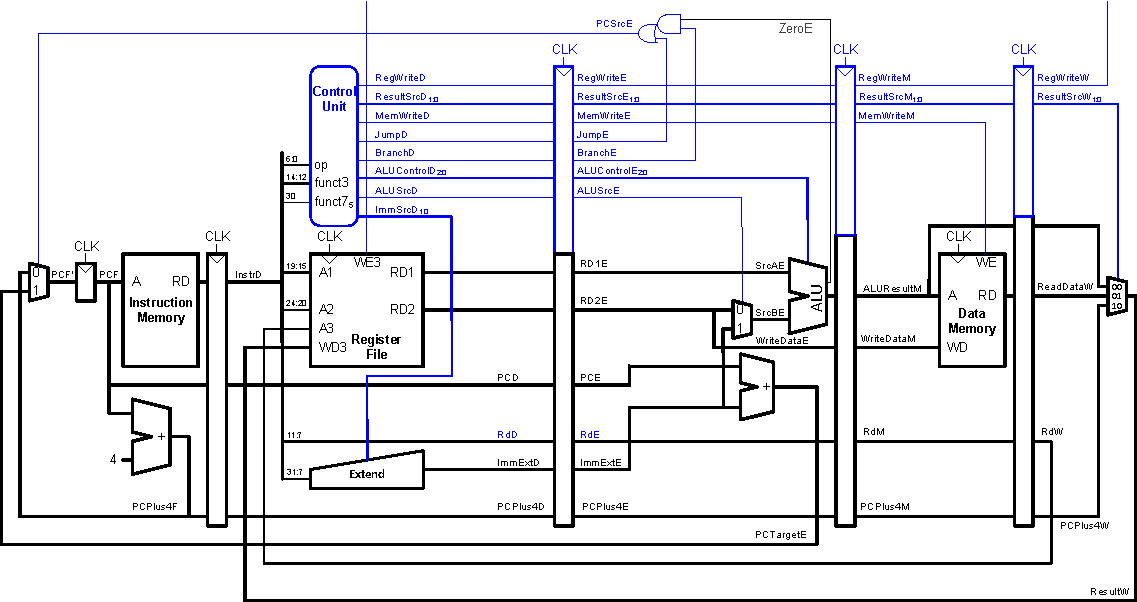
\includegraphics[width=0.85\textwidth]{w11_pipelined.pdf}
	\end{center}
\end{frame}

\begin{frame}[c, fragile]{Datenabhängigkeiten}{}
	\begin{columns}[c]
		\begin{column}{0.3\textwidth}
			{\ttfamily
				s1: lw {\only<1>{\color{red}}{t0}}, 0(a1)\\
				s2: lw t1, 0({\only<2>{\color{red}}{a0}})\\
				s3: add {\only<1>{\color{blue}}{t2}},  {\only<1>{\color{red}}{t0}}, s5\\
				s4: xor {\only<2,3>{\color{red}}{a0}},  {\only<1,2>{\color{blue}}{t2}}, a1\\
				s5: lw {\only<3>{\color{red}}{a0}}, 0(t1) \\
				s6: sub {\only<2>{\color{blue}}{t2}}, t3, t0  \\
			
		}
				\vspace{\baselineskip}\scriptsize{Mit * markierte Abhängigkeiten sind Datenkonflikte}

		\end{column}
		\begin{column}{0.4\textwidth}
			{\ttfamily
				\begin{tabular}{|c|c|c|c|c|c|}
					\hline
					i & F  & D  & E                                               & M                          & W                          \\
					\hline
					1 & s1 & -  & -                                               & -                          & -                          \\
					2 & s2 & s1 & -                                               & -                          & -                          \\
					3 & s3 & s2 & s1                                              & -                          & -                          \\
					4 & s4 & s3 & s2                                              & s1                         & -                          \\
					5 & s5 & s4 & \only<1>{\color{red}}{s3}                       & s2                         & \only<1>{\color{red}}{s1}  \\
					6 & s6 & s5 & \only<1>{\color{blue}}\only<2>{\color{red}}{s4} & \only<1>{\color{blue}}{s3} & \only<2>{\color{red}}{s2}  \\
					7 & ?  & s6 & \only<3>{\color{red}}{s5}                       & \only<3>{\color{red}}{s4}  & s3                         \\
					8 & ?  & ?  & \only<2>{\color{blue}}{s6}                      & s5                         & \only<2>{\color{blue}}{s4} \\
					\hline
				\end{tabular}
			}
		\end{column}
		\begin{column}{0.3\textwidth}
			\only<1,2>{Read after Write (RAW):
			{\ttfamily
			\begin{enumerate}[i.]
				\item s3, s1, t0*
				\item s4, s3, t2*
				\item s5, s2, t1
				\item s6, s1, t0
			\end{enumerate}
			}
			\vspace{\baselineskip}
			}
			\only<2,3>{Write after Read (WAR):
			{\ttfamily
			\begin{enumerate}[i.]
				\setcounter{enumi}{4}
				\item s4, s1, a1
				\item s4, s2, a0
				\item s5, s2, a0
				\item s6, s4, t2

			\end{enumerate}
			}
			\vspace{\baselineskip}
			}
			\only<3>{Write after Write (WAW):
			{\ttfamily
			\begin{enumerate}[i.]
				\setcounter{enumi}{8}
				\item s5, s4, a0
				\item s6, s3, t2
			\end{enumerate}
			}
			}
		\end{column}
	\end{columns}
\end{frame}

\begin{frame}[c, fragile]{Datenkonflikte}{}
	\begin{itemize}
		\item Daten\textit{abhängigkeiten}: RAW, WAR, WAW
		\item Pipelinekonflikte: Datenkonflikte (data hazards) und Steuerkonflikte (control hazards)
		\item Daten\textit{konflikte} können nur bei RAW auftreten (müssen aber nicht): Abhängige Instruktion ist in der Execute-Phase, aber das Ergebnis wurde noch nicht zurückgeschrieben
		\item Steuerkonflikte treten bei Änderung des Kontrollflusses auf (branches, jumps)
	\end{itemize}
\end{frame}

\begin{frame}[c, fragile]{Lösung von Konflikten}
	Bei \textbf{data hazards} müssen mindestens \textbf{3 Befehle} zwischen zwei Instruktionen mit RAW-Abhängigkeit stehen:
	\begin{itemize}
		\item NOPs (Stalling)
		\item Befehlsumordnung (ohne Änderung der Semantik)
		\item Forwarding: noch nicht zurückgeschriebenes Ergebnis kann von der ALU direkt an den nächsten Befehl gegeben werden, falls dieser das Ergebnis benötigt
	\end{itemize}
	\vspace{0.5cm}
	Bei \textbf{control hazards} müssen mindestens \textbf{2 Befehle} zwischen der Sprungentscheidung und möglicherweise falsch geladenen Instruktion stehen.
	\begin{itemize}
		\item NOPs (Stalling)
		\item Branch Prediction (statisch/dynamisch): Falls Vorhersage falsch, müssen geladene Instruktionen entfernt werden
	\end{itemize}
	\vspace{0.5cm}
	weitere Konzepte: Out-of-Order-Execution, Register Renaming, \ldots
\end{frame}

\begin{frame}[c, fragile]{Forwarding}{}
	\begin{center}
		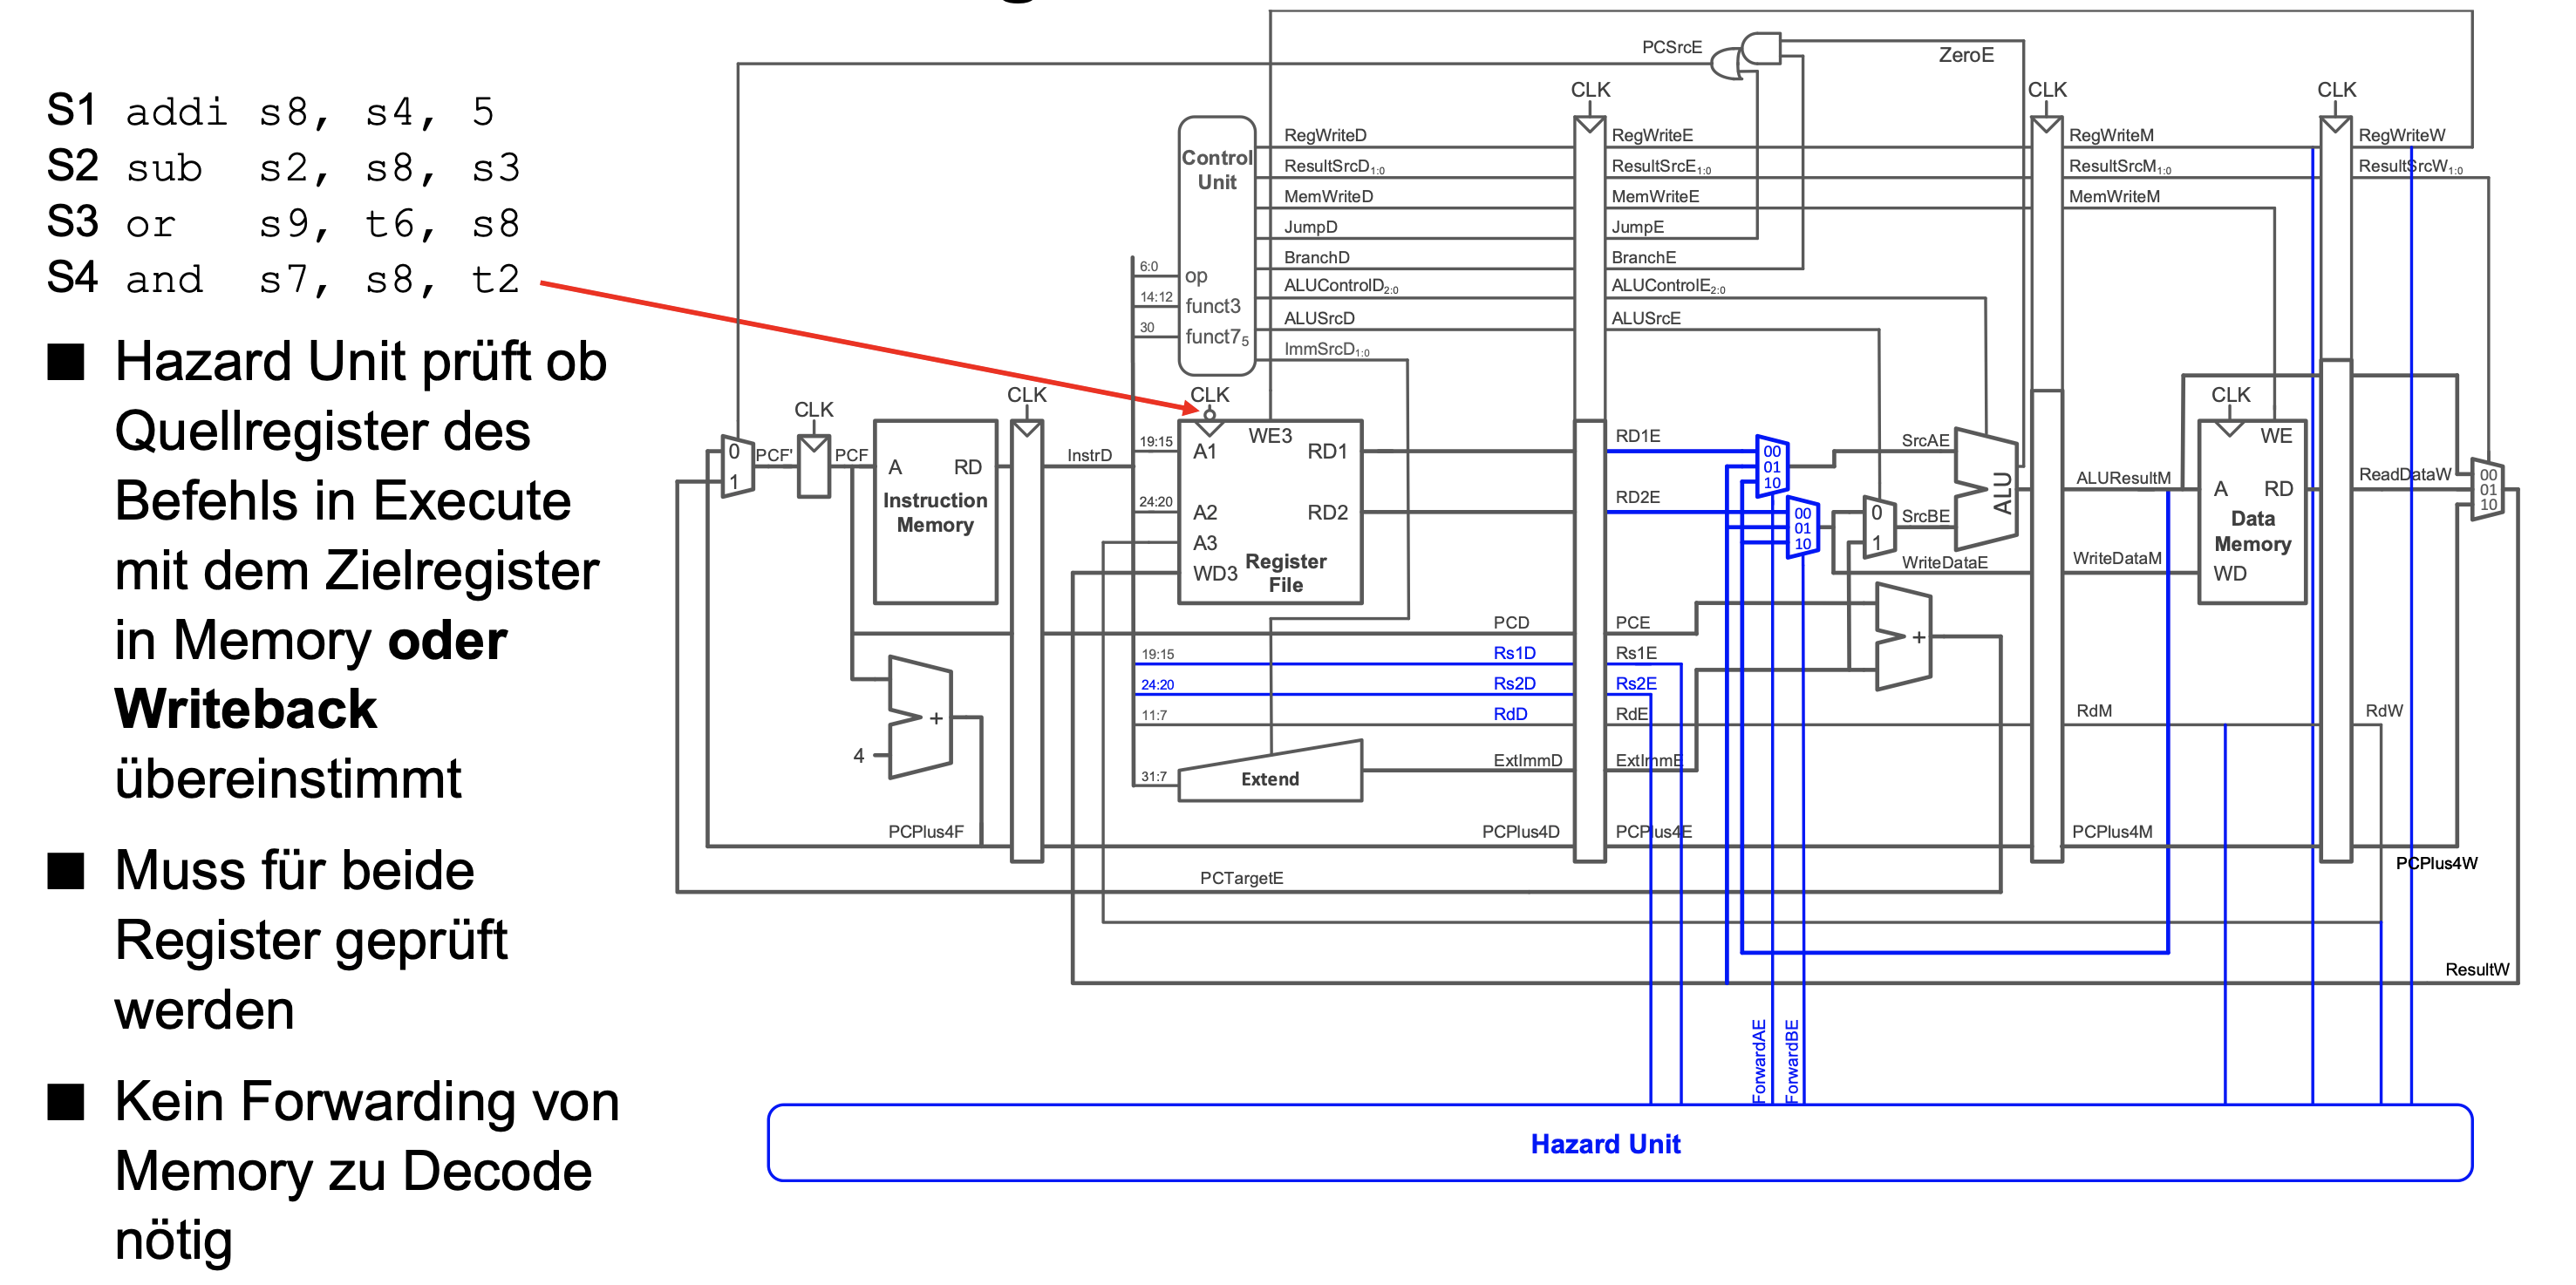
\includegraphics[width=0.9\textwidth]{w11_forwarding.png}		
	\end{center}
\end{frame}

\begin{frame}[c]{Aufgabe: Pipelining}{}
	Wieviele Zyklen benötigt die Ausführungen des folgenden Programms auf dem Pipelining Prozessor mit Hazard Unit ohne weitere Optimierungen:  \\
	\vspace{0.5cm}
	s1 \hspace{15mm} addi t1, zero, 52 \\
	s2 \hspace{15mm} addi t0, t1, -4    \\
	s3 \hspace{15mm} jal s4    \\
	s4 \hspace{15mm} lw t3, 16(t0)      \\
	s5 \hspace{15mm} sw t3, 20(t0)      \\
	s6 \hspace{15mm} xor t2, t0, t3     \\
	s7 \hspace{15mm} or t2, t2, t3      \\

\end{frame}

\begin{frame}[c]{Lösung: Pipelining}{}
	Wieviele Zyklen benötigt die Ausführungen des folgenden Programms auf dem Pipelining Prozessor mit Hazard Unit ohne weitere Optimierungen:  \\
	\vspace{0.5cm}
	\begin{columns}[c]
		\begin{column}{0.5\textwidth}
			s1 \hspace{15mm} addi t1, zero, 52 \\
			s2 \hspace{15mm} addi t0, t1, -4    \\
			s3 \hspace{15mm} jal s6    \\
			s4 \hspace{15mm} lw t3, 16(t0)      \\
			s5 \hspace{15mm} sw t3, 20(t0)      \\
			s6 \hspace{15mm} xor t2, t0, t3     \\
			s7 \hspace{15mm} or t2, t2, t3      \\
				\end{column}
		\begin{column}{0.5\textwidth}
			\begin{center}
				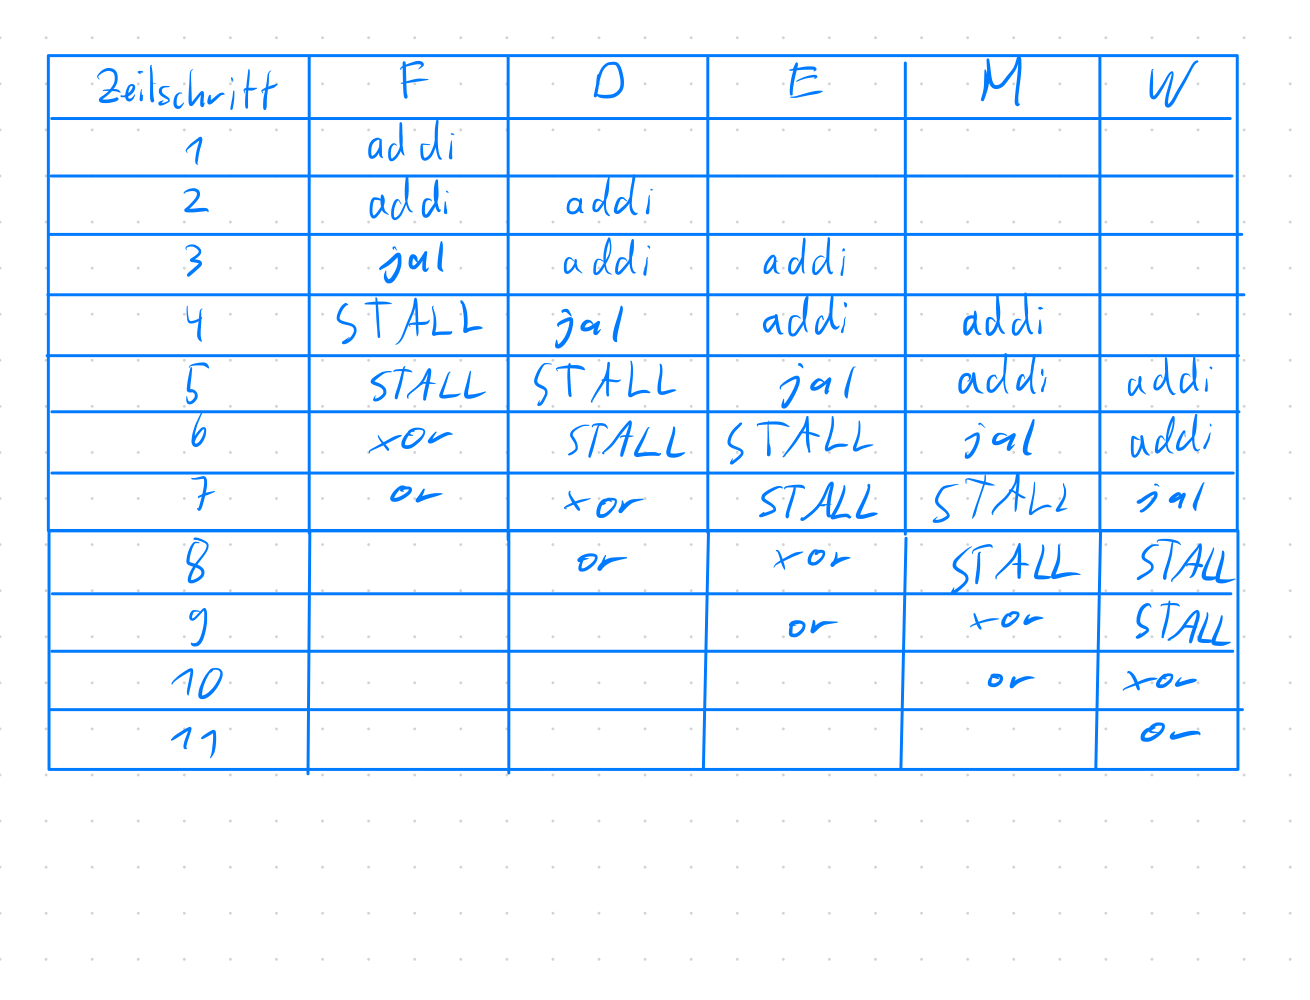
\includegraphics[width=1.0\textwidth]{w14_pipelining.jpeg}
			\end{center}
		\end{column}
	\end{columns}
\end{frame}

% --------------- PARALLELISIERUNG---------------------------------

\begin{frame}[c]{Wiederholung}{}
	\begin{center}
	  \LARGE Parallelisierung
	\end{center}
\end{frame}

\newcommand\mesipic[1][5]{
	\begin{tikzpicture}
		\tikzset{every node/.style={},
			label/.style={draw=none},
			local/.style={},
			remote/.style={blue},
			read/.style={dashed,->},
			write/.style={->}
		}

		\def\spacing{2.5cm}
		\def\legSpacing{1cm}

		\node[state] (m) {$M$};
		\node[state] (e) [right=\spacing of m] {$E$};
		\node[state] (s) [below=\spacing of m] {$S$};
		\node[state] (i)  [below=\spacing of e] {$I$};

		% local read
		\ifthenelse{#1 = 1 \or #1 = 5}{
			\path[local, read, every node/.style={execute at begin node=$, execute at end node=$}]
			(m) edge [loop above] node {r} ()
			(e) edge [loop above] node {r} ()
			(s) edge [loop below] node {r} ()
			(i) edge [bend left, below] node {r} (s)
			(i) edge [bend right, right] node {r} (e);
			test
		}{}

		% local write
		\ifthenelse{#1 = 2 \or #1 = 5}{
			\path[local, write, every node/.style={execute at begin node=$, execute at end node=$}]
			(m) edge [loop left] node {w} ()
			(e) edge [bend right, above] node {w} (m)
			(s) edge [bend left, left] node {w} (m)
			(i) edge [bend right, above] node {w} (m);
		}{}

		% remote read
		\ifthenelse{#1 = 3 \or #1 = 5}{
			\path[remote, read, every node/.style={execute at begin node=$, execute at end node=$}]
			(m) edge [bend left, right] node {r} (s)
			(e) edge [right] node {r} (s)
			(s) edge [loop left] node {r} ()
			(i) edge [loop below] node {r} ();
		}{}

		% remote write
		\ifthenelse{#1 = 4 \or #1 = 5}{
			\path[remote, write, every node/.style={execute at begin node=$, execute at end node=$}]
			(m) edge [left] node {w} (i)
			(e) edge [bend right, left] node {w} (i)
			(s) edge [bend left, above] node {w} (i)
			(i) edge [loop right] node {w} ();
		}{}

		\ifthenelse{#1 = 5}{
			\node[draw=none, minimum width=2cm, below=\legSpacing of s] (leg) {lokal};
			\node[draw=none, minimum width=2cm, below=\legSpacing of i] (leg2) {entfernt};
			\node[draw=none, minimum width=2cm, below=0.25*\legSpacing of leg] (leg3) {lesen};
			\node[draw=none, minimum width=2cm, below=0.25*\legSpacing of leg2] (leg4) {schreiben};

			\draw[very thick, local] (leg.west) -- ++(-0.5,0);
			\draw[very thick, remote](leg2.west) -- ++(-0.5,0);
			\draw[read, <-](leg3.west) -- ++(-0.5,0);
			\draw[, <-](leg4.west) -- ++(-0.5,0);
		}{}
	
	\node[draw=none, fit= (m) (e) (s) (i), inner sep=28pt] {};
	\end{tikzpicture}
}

\begin{frame}[c, fragile]{MSI/MESI}{}
	\begin{columns}[c]
		\begin{column}{0.5\textwidth}
			\begin{itemize}
				\item Mehrkernsysteme: Was wenn CPU1 und CPU2 beide ein Datum gecached haben und es modifizieren?\\$\rightarrow$ Cache-Inkonsistenzen
				\item Einführung von Zuständen für Cachezeilen
				\item CPUs hören jeweils die Zugriffe der anderen Kerne ab (\enquote{Bus Snooping})
				\item \textbf{M}odified, (\textbf{E}xclusive), \textbf{S}hared, \textbf{I}nvalid
				\item Exclusive-Bit ermöglicht kleineren Overhead wenn CPUs auf verschiedenen Cache-Blöcken arbeiten
			\end{itemize}
		\end{column}
		\begin{column}{0.5\textwidth}
			\begin{center}
				\resizebox{!}{0.8\textheight}{
					\mesipic[5]
				}
			\end{center}
		\end{column}
	\end{columns}
\end{frame}

\begin{frame}[c, fragile]{MESI: Übersicht}{}
	\begin{columns}[c]
		\begin{column}{0.5\textwidth}
			\begin{tabular}{cc}
				\resizebox{!}{0.45\textheight}{\mesipic[1]} & \resizebox{!}{0.45\textheight}{\mesipic[2]} \\
				\resizebox{!}{0.45\textheight}{\mesipic[3]} & \resizebox{!}{0.45\textheight}{\mesipic[4]}
			\end{tabular}
		\end{column}
		\begin{column}{0.4\textwidth}
			\begin{center}
				\resizebox{!}{0.8\textheight}{\mesipic[5]}
			\end{center}
		\end{column}
	\end{columns}
\end{frame}

\begin{frame}[c, fragile]{Speedup durch Parallelisierung}{}
	Mit $t_s$ sequentieller Programmteil, $t_p$ paralleler Programmteil, $n$ Anzahl CPU-Kerne,\\$T$ Ausführungszeit mit $n=1$:
	\begin{itemize}
		\item Amdahlsches Gesetz:
		      Gleiche Problemgröße, aufgeteilt auf mehrere Kerne $\rightarrow$ begrenzt durch sequentiellen Anteil
		      \[S_{\textrm{Amdahl}}(n)=\frac{T}{t_s+\frac{t_p}{n}}\]
		\item Gustafsons Gesetz:
		      Mehr Kerne können mehr berechnen: Größeres Problem$\rightarrow$ paralleler Anteil wächst mit Problemgröße, $t_s$ proportional kleiner
		      \[S_{\textrm{Gustafson}}(n)=\frac{t_s+n\cdot t_p}{T}\]
		\item Zwei verschiedene Perspektiven, abhängig von Problemszenario verschieden geeignet
	\end{itemize}
\end{frame}

\begin{frame}[c, fragile]{Roofline-Modell}{}
	\begin{columns}[c]
		\begin{column}{0.51\textwidth}
			\begin{itemize}
				\item Modellierung der maximalen Gesamtleistung
				\item X-Achse: Arithmetische Intensität (I)
				\begin{itemize}
					\item in FLOP pro Byte
					\item I = (Anzahl Rechenoperationen in FLOP) / (Speichertransfers in Byte)
					\item Abhängig vom Algorithmus
				\end{itemize}
				\item Y-Achse: Rechenleistung
				\begin{itemize}
					\item in FLOPS
					\item Abhängig vom Rechensystem
				\end{itemize}
				\item Diagonale: Max Speicherbandbreite
				\begin{itemize}
					\item y/x = (GFlop/s) / (Flop/Byte) = GB/s
				\end{itemize}
			\end{itemize}
		\end{column}
		\begin{column}{0.5\textwidth}
			\centering
			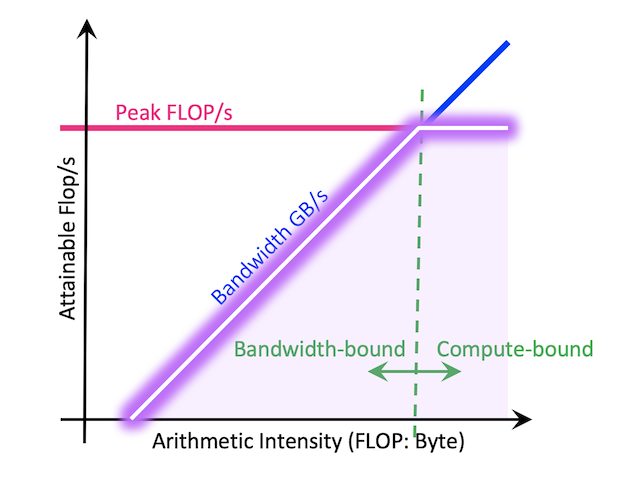
\includegraphics[width=\textwidth]{w10_roofline_google.png}
			\tiny{\href{https://docs.nersc.gov/tools/performance/roofline/}{Quelle}}
		\end{column}
	\end{columns}
\end{frame}

\begin{frame}[c]{Viel Erfolg!}{}
  \begin{center}
	Und für den Rest des Semesters überlegen wir uns noch was anderes. Bis dahin macht kein Schieß, wir sehen uns nächste Woche https://tum.live/w/ws24EidR/50024?t=5988
	\LARGE Ich wünsche euch viel Erfolg bei all euren Klausuren ;)
  \end{center}
\end{frame}
\end{document}